%% ============================================================================
%%  CodeSentinel -- research paper (IEEE conference, two-column)
%%  Build:  latexmk -pdf main.tex        (uses biber for the bibliography)
%%  Overleaf: set "main.tex" as the main document, compiler = pdfLaTeX.
%% ============================================================================
\documentclass[conference]{IEEEtran}
\IEEEoverridecommandlockouts

% --- Encoding & fonts -------------------------------------------------------
\usepackage[T1]{fontenc}
\usepackage[utf8]{inputenc}
\usepackage{microtype}

% --- Graphics, colour, maths, tables --------------------------------------
\usepackage[dvipsnames]{xcolor}
% Shared diagram palette (matches the product UI).
\definecolor{csslate}{HTML}{475569}
\definecolor{csink}{HTML}{0F172A}
\definecolor{csblue}{HTML}{2563EB}
\definecolor{csbluebg}{HTML}{EEF3FF}
\definecolor{csgraybg}{HTML}{F1F5F9}
\definecolor{csamber}{HTML}{D97706}
\definecolor{csamberbg}{HTML}{FEF3E2}
\definecolor{csgreen}{HTML}{059669}
\definecolor{csgreenbg}{HTML}{E7F6EF}
\definecolor{csred}{HTML}{DC2626}
\definecolor{csredbg}{HTML}{FCEBEB}
\usepackage{graphicx}
\graphicspath{{figures/}{figures/screens/}{figures/diagrams/}}
\usepackage{amsmath,amssymb}
\usepackage{booktabs}
\usepackage{array}
\usepackage{multirow}
\usepackage{tabularx}
\usepackage{makecell}
\usepackage{subcaption}
\usepackage{balance}

% --- Diagrams -------------------------------------------------------------
\usepackage{tikz}
\usetikzlibrary{positioning,shapes.geometric,arrows.meta,calc,fit,backgrounds,
                decorations.pathreplacing}

% --- Code / finding listings -------------------------------------------------
\usepackage{listings}
\definecolor{codebg}{HTML}{0B1220}
\definecolor{codekw}{HTML}{7AA2F7}
\definecolor{codestr}{HTML}{9ECE6A}
\definecolor{codecmt}{HTML}{9AA5B1}
\lstdefinestyle{finding}{
  basicstyle=\ttfamily\scriptsize\color{white},
  backgroundcolor=\color{codebg},
  keywordstyle=\color{codekw}\bfseries,
  stringstyle=\color{codestr},
  commentstyle=\color{codecmt}\itshape,
  breaklines=true, showstringspaces=false, columns=fullflexible,
  frame=single, framesep=4pt, rulecolor=\color{codebg},
  xleftmargin=4pt, xrightmargin=4pt, aboveskip=6pt, belowskip=4pt,
  language=Python
}

% --- Bibliography: clickable, IEEE-style references ------------------------
\usepackage[style=ieee,backend=biber,sorting=none,doi=true,url=true,isbn=false]{biblatex}
\addbibresource{references.bib}

% --- Hyperlinks: clickable citations, cross-references and URLs -----------
\usepackage[colorlinks=true,
            linkcolor=RoyalBlue,
            citecolor=BrickRed,
            urlcolor=Teal,
            breaklinks=true,
            bookmarksnumbered=true]{hyperref}
\usepackage[capitalise,nameinlink]{cleveref}
\crefname{table}{Table}{Tables}
\crefname{figure}{Fig.}{Figs.}
\Crefname{figure}{Figure}{Figures}
\crefname{equation}{Eq.}{Eqs.}
\crefname{section}{Section}{Sections}

% --- Convenience macros ----------------------------------------------------
\usepackage{xspace}
\newcommand{\cs}{\textsc{CodeSentinel}\xspace}
\newcommand{\phindex}{\textit{Project Health Index}\xspace}
\newcommand{\vellum}{\textit{Vellum}\xspace}

\begin{document}

\title{\cs: A Local-First Platform for Large-Language-Model-Assisted\\
Static and Dynamic Source-Code Security Auditing}

\author{
  \IEEEauthorblockN{Ali Hamza}
  \IEEEauthorblockA{%
    \textit{Department of Computer Science}\\
    \textit{[Institution]}\\
    [City, Country]\\
    [author email]}
}

\maketitle

\begin{abstract}
Modern software teams increasingly depend on two classes of assistive
technology to keep source code secure: static application security
testing (SAST) and, more recently, large language models (LLMs) used for
code review and vulnerability triage. Both are usually delivered as cloud
services, which obliges an organisation to transmit proprietary source
code to a third party and complicates adoption in regulated or air-gapped
environments. This paper presents \cs, a local-first desktop platform that
unifies pattern-based static analysis, containerised dynamic execution,
and on-device LLM reasoning into a single privacy-preserving workflow for
auditing the security and structural health of a source-code repository.
Every stage runs on the developer's machine: pattern detectors and a
cyclomatic-complexity engine operate in process, a quantised
\mbox{Llama~3.2} model performs semantic review inside a local container,
and a resource-limited Docker sandbox exercises the project at runtime.
Findings from the three modalities are fused, de-duplicated, and combined
with software metrics into a single \phindex. We describe the
architecture, the analysis pipeline, and the scoring model, and we
present the twelve-screen graphical interface through which a developer
drives and inspects an audit. A worked case study on a representative
retrieval-augmented-generation service ($47$ files, ${\sim}5.2$~KLOC)
shows the platform surfacing $20$ findings spanning credential handling,
prompt and query injection, unsafe deserialisation, and server-side
request forgery, alongside five cyclomatic hot-spots and a moderate
composite risk score, while completing end to end in under a minute and
without a single outbound network request. We discuss the trade-offs of
local inference, the limitations of the current prototype, and directions
for a larger empirical evaluation.
\end{abstract}

\begin{IEEEkeywords}
Static application security testing, large language models, on-device
inference, dynamic analysis, cyclomatic complexity,
retrieval-augmented generation, privacy-preserving software tools,
developer tooling.
\end{IEEEkeywords}


\section{Introduction}
\label{sec:intro}

Source code is now the primary attack surface of most organisations. A
single hard-coded credential, an unsanitised path into a query builder,
or an unsafe deserialisation call can compromise an entire deployment,
and the categories of weakness responsible have remained remarkably
stable for two decades~\cite{owasp2021,mitrecwe}. Two families of tools
have emerged to help developers find such defects before release. Static
application security testing (SAST) analyses code without executing it,
using pattern matching, data-flow, and taint tracking to flag suspicious
constructs~\cite{chess2004,ayewah2008,yamaguchi2014}. More recently,
large language models (LLMs) trained on code have been applied to review,
vulnerability detection, and repair, offering a form of semantic
reasoning that rule-based analysers lack~\cite{chen2021codex,pearce2023,
khoury2023}.

Despite their complementary strengths, both families share a deployment
assumption that is increasingly at odds with how sensitive code is
governed: they run in the cloud. Commercial SAST platforms upload the
repository to a hosted analysis backend, and virtually every capable
code-reasoning LLM is accessed through a remote API. For teams working on
proprietary algorithms, unreleased products, defence or medical software,
or anything subject to data-residency rules, transmitting the source
tree off the premises is either prohibited outright or requires a
contractual and architectural effort that discourages routine use. The
same barrier blocks adoption in genuinely air-gapped settings. The
practical consequence is that the developers who arguably need rigorous
auditing most are the least able to use the current generation of
assistive tools.

A second, well-documented problem is that developers frequently abandon
static analysers because the tools do not fit their workflow: results
arrive out of context, the signal-to-noise ratio is poor, and the
interface makes triage tedious~\cite{johnson2013,nachtigall2022}. A tool
that solves the privacy problem but reproduces the usability problem will
not be adopted either.

This paper describes \cs, a desktop application that addresses both
concerns. \cs performs a complete security and structural audit of a
repository \emph{entirely on the developer's own machine}. It combines
three analysis modalities---pattern-based static detection, on-device
LLM semantic review, and containerised dynamic execution---behind a
single graphical workflow, and it aggregates their output, together with
classical software metrics, into one interpretable score. The LLM
component runs a quantised \mbox{Llama~3.2} model inside a local
container via Ollama~\cite{ollama,touvron2023llama2}; the dynamic
component builds and runs the project inside a resource-limited Docker
sandbox~\cite{merkel2014docker}. No stage of the pipeline opens an
outbound network connection, and the application exposes an explicit
offline indicator so that this property is visible to the user.

\smallskip
\noindent\textbf{Contributions.} This paper makes the following
contributions:
\begin{itemize}
  \item A \emph{local-first architecture} that co-locates pattern-based
        SAST, an on-device code-reasoning LLM, a cyclomatic-complexity
        engine, and a container sandbox in a single desktop process, with
        a hard no-egress boundary (\cref{sec:method}).
  \item A \emph{finding-fusion and composite-scoring} method that
        reconciles rule-based and model-based findings and folds them,
        with structural metrics, into a single \phindex\ and a set of
        interpretable risk bands (\cref{sec:fusion,sec:risk}).
  \item A \emph{task-oriented interface} of twelve coordinated screens
        that let a developer configure an audit, watch it run, and triage
        results in the context of the offending source
        (\cref{sec:interface}).
  \item A \emph{worked case study} on a representative
        retrieval-augmented-generation (RAG) service that exercises the
        weakness classes now specific to LLM-integrated
        applications~\cite{owaspllm2025,greshake2023}, and a discussion of
        where local inference helps and where it costs recall
        (\cref{sec:results,sec:discussion}).
\end{itemize}

\smallskip
\noindent The remainder of the paper is organised as follows.
\Cref{sec:related} surveys static and dynamic analysis, software metrics,
and the use of language models for code and security.
\Cref{sec:method} presents the architecture, the analysis pipeline, and
the scoring model. \Cref{sec:interface} walks through the product
interface. \Cref{sec:results} reports the case study. \Cref{sec:discussion}
discusses trade-offs and threats to validity, and \Cref{sec:conclusion}
concludes.

\section{Background and Related Work}
\label{sec:related}

The idea that a machine should read code for defects is old, and its
history is a sequence of solutions each of which created the next
problem. The earliest security-relevant static analysers were syntactic:
lint-style checks and, later, bug-pattern detectors such as
FindBugs~\cite{ayewah2008}. They were cheap to run and caught real
mistakes, which established that automated inspection was worthwhile at
all. Their weakness was equally clear, a purely local pattern cannot see
how a tainted value flows across functions, so the field moved to
inter-procedural data-flow and taint analysis. Coverity showed that this
could be done over hundreds of millions of lines of industrial
code~\cite{bessey2010}, Infer brought a compositional formulation to a
comparable scale~\cite{distefano2019}, and Chess and McGraw framed the
whole activity as a security discipline rather than a quality
one~\cite{chess2004}. Depth, however, came with two costs: substantial
engineering to deploy, and a false-positive burden large enough that
managing it became a product in itself. Studies of practitioners found
that developers abandon static analysers not because the tools lack
power, but because results arrive out of context, the noise is high, and
triage does not fit the way people work~\cite{johnson2013,nachtigall2022}.

The response to the rule-authoring bottleneck was to make rules a
first-class, shareable artefact. Yamaguchi \textit{et~al.}\ modelled a
program as a code property graph so that a vulnerability could be
expressed as a graph query~\cite{yamaguchi2014}, and CodeQL turned such
queries into a declarative language with a community
library~\cite{avgustinov2016}; lighter open tools such as
Semgrep~\cite{semgrep} and Bandit~\cite{bandit} put custom rules in reach
of ordinary developers. This solved shareability but not the underlying
limit: a rule, however elegant, encodes a pattern the author already
anticipated, and every new class of weakness needs a new rule. In
parallel, a different line of work summarised a program's health as a
number rather than a list of defects. McCabe's cyclomatic
complexity~\cite{mccabe1976} correlates with defect density and test
effort, and the Maintainability Index folded it together with size and
volume into a single figure~\cite{coleman1994}. These metrics are useful
as a triage signal, but a scalar does not localise or explain a
vulnerability, it only says where to look harder.

Because static reasoning is necessarily incomplete, execution-based
methods developed alongside it. Fuzzing became the dominant automated
bug-finding technique for native code~\cite{manes2021}, and container
isolation made it routine to run unknown or untrusted software with
bounded privileges~\cite{merkel2014docker}. Dynamic analysis finds bugs
that static analysis cannot, but it needs harnesses, it needs time, and
it covers business logic poorly, so it complements rather than replaces
the static passes.

The next shift was semantic. LLMs trained on source code could, for the
first time, reason about a program's intent rather than its
syntax~\cite{chen2021codex}, and researchers quickly turned them toward
security. Pearce \textit{et~al.}\ measured how often code \emph{generated}
by an assistant is insecure~\cite{pearce2022} and then showed that an LLM
can \emph{repair} vulnerabilities zero-shot~\cite{pearce2023}; Khoury
\textit{et~al.}\ found that a large fraction of ChatGPT-produced snippets
contain exploitable flaws~\cite{khoury2023}. Learned detectors such as
Devign~\cite{zhou2019devign} and LineVul~\cite{fu2022linevul} predicted
vulnerable functions and lines directly. The capability was real, but two
new problems came with it. First, the reported accuracy of learned
detectors proved highly sensitive to the quality of the training and
evaluation data, and drops sharply across
projects~\cite{steenhoek2023,croft2023}, which argues for keeping a human
in the loop rather than trusting a verdict. Second, and more
fundamental for practice, the models capable of this reasoning are
reached through hosted APIs, so using them re-introduces exactly the
confidentiality and cost problems that on-premises static analysis had
avoided.

The analysis target then moved as well. As applications began embedding
LLMs, prompt injection emerged as a weakness class in its own
right, direct manipulation of the instruction stream~\cite{perez2022ignore}
and indirect injection through retrieved content~\cite{greshake2023}, and
was codified in the OWASP Top~10 for LLM
Applications~\cite{owaspllm2025}. Retrieval-augmented
generation~\cite{lewis2020rag} is especially exposed, because it adds a
document loader, an embedding store, and a reranker, each a fresh sink for
untrusted input. An analyser built today has to cover this class, not
just the classical one.

The final piece is what makes a different design possible. Open model
families such as LLaMA and Llama~2~\cite{touvron2023llama,touvron2023llama2},
together with efficient quantised inference runtimes like
Ollama~\cite{ollama}, now let a multi-billion-parameter model run on a
laptop at interactive speed. The technical reason the semantic step had
to live in the cloud has therefore gone away.

\cs\ is the point where these threads meet. Prior work advanced one axis
at a time and paid for it on another: depth of analysis at the expense of
usability, semantic power at the expense of confidentiality and cost,
breadth of coverage at the expense of integration. \cs\ instead runs
pattern-based SAST, a cyclomatic-complexity engine, an on-device
\mbox{Llama~3.2} semantic reviewer, and a containerised dynamic pass
together on the developer's machine, behind one interface and one
transparent \phindex, with a hard no-egress boundary. It gives up
frontier-model scale to do so, and manages that trade by keeping the
model advisory and always shown next to a corroborating deterministic
rule and the offending source. \Cref{tab:litreview} summarises the works
above, the advance each made, and the limitation \cs\ is designed to
carry forward.

\begin{table*}[!tbp]
  \centering
  \caption{The evolution of automated code security analysis: what each
           line of work advanced, and the limitation it left open.}
  \label{tab:litreview}
  \renewcommand{\arraystretch}{1.25}
  \small
  \begin{tabularx}{\textwidth}{@{}p{0.20\textwidth} X X@{}}
    \toprule
    \textbf{Study / system} & \textbf{Advance and key findings} &
    \textbf{Limitation left open} \\
    \midrule

    FindBugs; bug patterns \cite{ayewah2008} &
      Simple syntactic patterns find real defects at very low cost;
      established automated inspection as worthwhile. &
      Local patterns cannot follow a tainted value across
      procedures; shallow coverage of semantic bugs. \\

    Coverity at scale \cite{bessey2010} &
      Inter-procedural analysis runs on $10^8$-line industrial
      codebases and finds serious defects in the field. &
      Heavy deployment effort; false-positive triage becomes a
      product in itself. \\

    Infer / compositional analysis \cite{distefano2019} &
      Compositional summaries make deep analysis scale and fit CI. &
      Targets specific bug classes; still rule-/spec-bound. \\

    Developer studies \cite{johnson2013,nachtigall2022} &
      Identify \emph{why} SAST is abandoned: out-of-context results,
      noise, poor workflow fit. &
      Diagnose the adoption problem but propose no tool. \\

    Code property graphs \cite{yamaguchi2014} &
      Represent code as a graph so a vulnerability is a query;
      reusable across a codebase. &
      Requires expert query authoring for each weakness class. \\

    CodeQL \cite{avgustinov2016} &
      Declarative, shareable security queries with a community
      library. &
      A rule encodes a pattern the author anticipated; cannot infer
      intent. \\

    Cyclomatic complexity;
    Maintainability Index \cite{mccabe1976,coleman1994} &
      A structural-health scalar that correlates with defect density
      and test effort. &
      A number does not localise or explain a vulnerability. \\

    Fuzzing survey \cite{manes2021} &
      Execution finds bugs static analysis misses; now the dominant
      automated technique for native code. &
      Needs harnesses and time; weak coverage of business logic. \\

    Codex / LLMs for code \cite{chen2021codex} &
      Models trained on code reason about \emph{intent}, not just
      syntax. &
      General-purpose, not security-tuned; capable variants are
      hosted only. \\

    Copilot / ChatGPT code security
    \cite{pearce2022,khoury2023} &
      Quantify how often assistant-\emph{generated} code is
      insecure. &
      Evaluate the generation side, not a defensive analysis tool;
      prompts still leave the machine. \\

    Devign; LineVul
    \cite{zhou2019devign,fu2022linevul} &
      Learned models predict vulnerable functions / lines directly. &
      Accuracy tied to noisy datasets; weak cross-project
      generalisation. \\

    Zero-shot vulnerability repair \cite{pearce2023} &
      A capable LLM can repair vulnerabilities with no
      task-specific training. &
      Needs a frontier (hosted) model; unreliable without an oracle. \\

    Data-quality critiques
    \cite{steenhoek2023,croft2023} &
      Show DL vulnerability-detection results are inflated by
      label/duplication issues. &
      Argue against trusting a verdict; motivate human-in-the-loop. \\

    Prompt injection; OWASP LLM Top~10
    \cite{perez2022ignore,greshake2023,owaspllm2025} &
      Define a new weakness class (direct and retrieval-borne) that
      analysers must now cover. &
      RAG systems \cite{lewis2020rag} are especially exposed; the
      analysis target itself has moved. \\

    Open quantised models; Ollama
    \cite{touvron2023llama,touvron2023llama2,ollama} &
      Multi-billion-parameter models run on a laptop at interactive
      speed. &
      Smaller than frontier models; recall of subtle,
      cross-function bugs is lower. \\

    \midrule
    \textbf{\cs\ (this work)} &
      Runs pattern SAST, complexity metrics, an on-device
      \mbox{Llama~3.2} reviewer, and a container sandbox together
      behind one interface and one transparent score, with a hard
      no-egress boundary. &
      Trades frontier-model scale for locality; the model is kept
      advisory and corroborated by deterministic rules. \\
    \bottomrule
  \end{tabularx}
\end{table*}


\section{System Design and Methodology}
\label{sec:method}

\subsection{Design Goals}
\cs\ was built around four goals. \textbf{(G1) No network egress:} a
complete audit must run with the machine's network interface disabled, so
that no code, prompt, or result is ever transmitted. \textbf{(G2)
Multi-modal:} pattern analysis, structural metrics, semantic (LLM)
review, and dynamic execution should contribute to one result rather than
living in separate tools. \textbf{(G3) Context-preserving triage:} every
finding must be inspectable next to the exact source that produced it.
\textbf{(G4) One number, honestly derived:} the platform should output a
single interpretable health score whose computation is fully disclosed.

\subsection{Architecture}
\label{sec:arch}
\begin{figure*}[t]
  \centering
  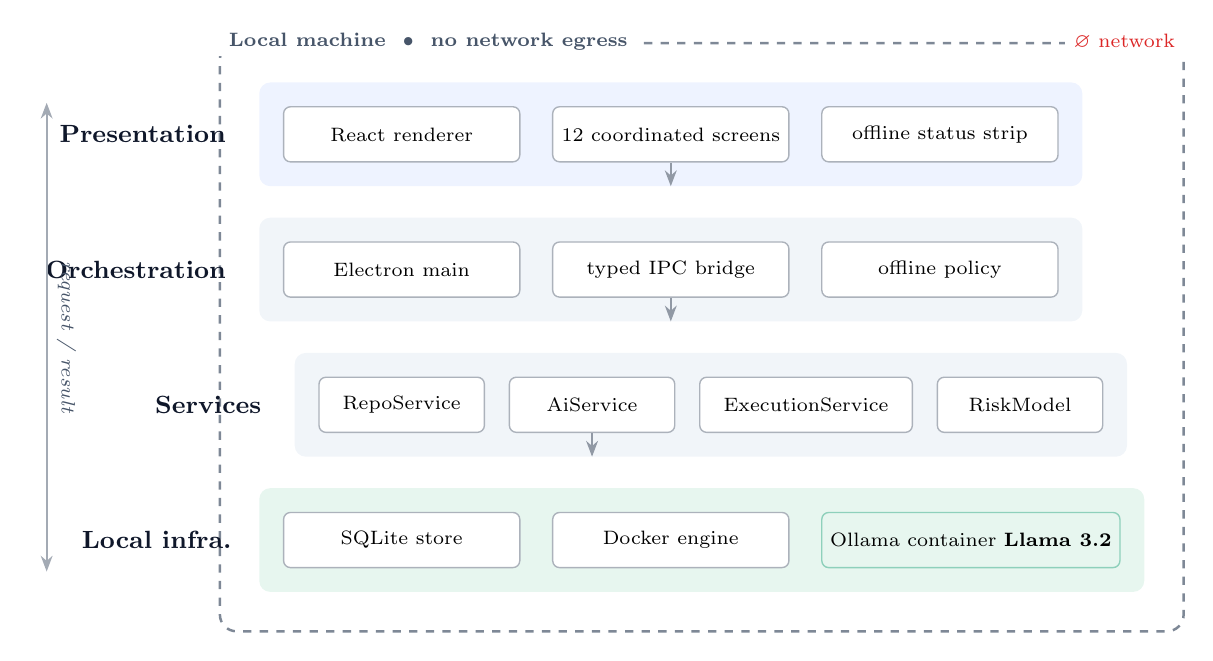
\begin{tikzpicture}[
      font=\footnotesize,
      chip/.style={rounded corners=2.5pt, draw=csslate!45, fill=white,
                   line width=0.5pt, minimum height=7mm, minimum width=30mm,
                   align=center, font=\scriptsize, inner sep=3pt},
      lyr/.style={font=\small\bfseries, color=csink, anchor=east,
                  align=right, text width=24mm},
      dn/.style={-{Stealth[length=2mm]}, draw=csslate!60, line width=0.8pt},
    ]

    % ---------- Presentation ----------
    \node[chip] (p1) {React renderer};
    \node[chip, right=4mm of p1] (p2) {12 coordinated screens};
    \node[chip, right=4mm of p2] (p3) {offline status strip};
    \node[lyr] at ([xshift=-6mm]p1.west) {Presentation};

    % ---------- Orchestration ----------
    \node[chip, below=10mm of p1] (o1) {Electron main};
    \node[chip, right=4mm of o1] (o2) {typed IPC bridge};
    \node[chip, right=4mm of o2] (o3) {offline policy};
    \node[lyr] at ([xshift=-6mm]o1.west) {Orchestration};

    % ---------- Services ----------
    \node[chip, below=10mm of o1, minimum width=21mm] (s1) {RepoService};
    \node[chip, right=3mm of s1, minimum width=21mm] (s2) {AiService};
    \node[chip, right=3mm of s2, minimum width=27mm] (s3) {ExecutionService};
    \node[chip, right=3mm of s3, minimum width=21mm] (s4) {RiskModel};
    \node[lyr] at ([xshift=-6mm]s1.west) {Services};

    % ---------- Local infrastructure ----------
    \node[chip, below=10mm of s1] (i1) {SQLite store};
    \node[chip, right=4mm of i1] (i2) {Docker engine};
    \node[chip, right=4mm of i2, fill=csgreenbg, draw=csgreen!45] (i3)
      {Ollama container \textbf{Llama 3.2}};
    \node[lyr] at ([xshift=-6mm]i1.west) {Local infra.};

    % ---------- layer backdrops ----------
    \begin{scope}[on background layer]
      \node[rounded corners=4pt, fill=csbluebg,  fit=(p1)(p3), inner sep=3mm] {};
      \node[rounded corners=4pt, fill=csgraybg,  fit=(o1)(o3), inner sep=3mm] {};
      \node[rounded corners=4pt, fill=csgraybg,  fit=(s1)(s4), inner sep=3mm] {};
      \node[rounded corners=4pt, fill=csgreenbg, fit=(i1)(i3), inner sep=3mm] {};
    \end{scope}

    % ---------- flow ----------
    \draw[dn] (p2.south) -- ++(0,-3mm);
    \draw[dn] (o2.south) -- ++(0,-3mm);
    \draw[dn] (s2.south) -- ++(0,-3mm);
    \draw[{Stealth[length=2mm]}-{Stealth[length=2mm]}, draw=csslate!50,
          line width=0.7pt]
      ([xshift=-30mm,yshift=4mm]p1.west) -- ([xshift=-30mm,yshift=-4mm]i1.west)
      node[midway, sloped, above, font=\scriptsize\itshape, color=csslate]
      {request / result};

    % ---------- no-egress boundary ----------
    \begin{scope}[on background layer]
      \node[draw=csslate!70, dashed, line width=0.9pt, rounded corners=6pt,
            fit=(p1)(p3)(i1)(i3), inner sep=8mm] (box) {};
    \end{scope}
    \node[anchor=west, font=\scriptsize\bfseries, color=csslate,
          fill=white, inner sep=2pt]
      at (box.north west) {\,Local machine\ \ $\bullet$\ \ no network egress\,};
    \node[anchor=east, font=\scriptsize, color=csred, fill=white, inner sep=2pt]
      at (box.north east) {\,$\varnothing$ network\,};

  \end{tikzpicture}
  \caption{\cs\ architecture. Four in-machine layers inside a hard
           no-egress boundary: a React presentation layer, an Electron
           orchestration layer, four analysis services, and local
           infrastructure hosting SQLite, the Docker engine, and the
           quantised \mbox{Llama~3.2} model. No stage opens an outbound
           connection.}
  \label{fig:architecture}
\end{figure*}


\cs\ is an Electron~\cite{electron} desktop application with a strict
main/renderer split. \Cref{fig:architecture} shows the four layers, all
resident on the developer's machine inside a no-egress boundary.

\begin{itemize}
 \item The \emph{presentation layer} is a React single-page application
 of twelve coordinated screens (\cref{sec:interface}). It holds no
 analysis logic; it issues typed requests over an
 inter-process-communication (IPC) bridge and renders results.
 \item The \emph{orchestration layer} (the Electron main process)
 validates each request, enforces the offline policy, and routes
 work to the services.
 \item The \emph{service layer} contains four in-process modules: a
 \textsc{RepoService} (checkout, file inventory, pattern
 detection, complexity), an \textsc{AiService} (prompt assembly,
 model I/O, finding extraction), an \textsc{ExecutionService}
 (Dockerfile synthesis, image build, sandboxed run, telemetry),
 and a \textsc{RiskModel} (fusion and scoring).
 \item The \emph{local infrastructure layer} comprises an embedded
 SQLite database for projects and findings, the host Docker
 engine, and an Ollama container hosting the quantised
 \mbox{Llama~3.2} weights~\cite{ollama,touvron2023llama2}.
\end{itemize}

\subsection{Analysis Pipeline}
\label{sec:pipeline}
\begin{figure*}[t]
  \centering
  \begin{tikzpicture}[
      font=\footnotesize,
      node distance=6mm,
      stage/.style={rounded corners=3pt, draw=csslate!45, fill=csgraybg,
                    line width=0.6pt, minimum height=9mm, minimum width=20mm,
                    align=center, inner sep=4pt},
      ana/.style={rounded corners=3pt, draw=csblue!45, fill=csbluebg,
                  line width=0.6pt, minimum height=8mm, minimum width=30mm,
                  align=center, inner sep=3pt, font=\scriptsize},
      out/.style={rounded corners=3pt, draw=csgreen!50, fill=csgreenbg,
                  line width=0.6pt, minimum height=9mm, minimum width=20mm,
                  align=center, inner sep=4pt},
      fl/.style={-{Stealth[length=2mm]}, draw=csslate!60, line width=0.8pt},
    ]

    \node[stage] (repo)  {Repository};
    \node[stage, right=of repo] (inv) {File\\inventory};

    % parallel analyses
    \node[ana, right=14mm of inv, yshift=10mm]  (pat) {Pattern scan\\\scriptsize(rules, CWE)};
    \node[ana, right=14mm of inv]               (cx)  {Complexity engine\\\scriptsize(McCabe $CC$)};
    \node[ana, right=14mm of inv, yshift=-10mm] (llm) {LLM review\\\scriptsize(Llama 3.2, schema)};

    \node[stage, right=14mm of cx] (fuse) {Finding\\fusion};
    \node[stage, right=of fuse]    (dyn)  {Dynamic\\sandbox};
    \node[stage, right=of dyn]     (risk) {Risk\\model};
    \node[out,   right=of risk]    (rep)  {Report\\\scriptsize PDF / JSON};

    \draw[fl] (repo) -- (inv);
    \draw[fl] (inv.east) -- (pat.west);
    \draw[fl] (inv.east) -- (cx.west);
    \draw[fl] (inv.east) -- (llm.west);
    \draw[fl] (pat.east) -- (fuse.west);
    \draw[fl] (cx.east)  -- (fuse.west);
    \draw[fl] (llm.east) -- (fuse.west);
    \draw[fl] (fuse) -- (dyn);
    \draw[fl] (dyn)  -- (risk);
    \draw[fl] (risk) -- (rep);

    \node[font=\scriptsize\itshape, color=csslate, above=1mm of pat] {in process};
    \node[font=\scriptsize\itshape, color=csslate, below=1mm of llm]
      {local container};

  \end{tikzpicture}
  \caption{The \cs\ analysis pipeline. A file inventory feeds three
           parallel analyses---pattern scanning and complexity in
           process, semantic review by the on-device model---whose
           output is fused (\cref{sec:fusion}), augmented by a sandboxed
           dynamic pass, and aggregated into the composite risk score and
           the exported report.}
  \label{fig:pipeline}
\end{figure*}


\Cref{fig:pipeline} shows the end-to-end pipeline. After a repository is
registered, \cs\ walks the working tree, applies language filters, and
produces a file inventory. Three analyses then run over that inventory;
the first two are in-process and the third is delegated to the local
model. \Cref{tab:modalities} maps each modality to the weakness
categories it is responsible for.

\begin{table}[t]
  \centering
  \caption{Analysis modalities and the weakness categories each is
           primarily responsible for.}
  \label{tab:modalities}
  \renewcommand{\arraystretch}{1.15}
  \small
  \begin{tabularx}{\columnwidth}{@{}l X@{}}
    \toprule
    \textbf{Modality} & \textbf{Primary responsibility} \\
    \midrule
    Pattern detection &
      Hard-coded secrets, injection sinks, unsafe deserialisation,
      request forgery, private-key material, missing authorisation
      (CWE-77/89/502/918/798)~\cite{mitrecwe}. \\
    Complexity engine &
      Per-function cyclomatic complexity, decision-point counts, and
      structural hot-spot ranking~\cite{mccabe1976}. \\
    LLM semantic review &
      Context-dependent issues: prompt-context handling, unbounded
      resource use, error-suppression, non-determinism, and design
      weaknesses specific to LLM-integrated
      applications~\cite{owaspllm2025}. \\
    Dynamic sandbox &
      Buildability, start-up and resource behaviour, and coarse runtime
      file/socket/process activity~\cite{merkel2014docker}. \\
    \bottomrule
  \end{tabularx}
\end{table}


\subsubsection{Pattern-based detection}
Each source file is scanned with a curated set of syntactic and
lightweight semantic rules targeting high-severity, low-ambiguity
classes: hard-coded secrets and high-entropy literals, command/SQL/prompt
injection sinks, unsafe deserialisation (e.g.\ \texttt{pickle.load} on
non-trusted input), server-side request forgery patterns, private-key
material, and missing-authorisation markers on privileged routes. Rules
carry a severity, a Common Weakness Enumeration
identifier~\cite{mitrecwe} where applicable, and a suggested remediation.

\subsubsection{Cyclomatic complexity engine}
For every function, \cs\ computes McCabe cyclomatic complexity $CC$ from
the control-flow graph~\cite{mccabe1976}, counts decision points, and
records the functions whose $CC$ exceeds a configurable budget as
\emph{structural hot-spots}. The mean complexity $\overline{CC}$ over all
analysed functions feeds the composite score (\cref{sec:risk}).

\subsubsection{On-device LLM semantic review}
\label{sec:llm}
The \textsc{AiService} sends each file (or, for large files, a bounded
window) to the local \mbox{Llama~3.2} model through the Ollama HTTP
endpoint on \texttt{127.0.0.1}. The prompt has three parts: a fixed
system preamble that defines the reviewer role and refusal policy; the
code under review, delimited so that its content cannot be interpreted as
instructions; and a response schema requesting a JSON array of findings
with \texttt{severity}, \texttt{title}, \texttt{line},
\texttt{description}, and \texttt{suggestedFix} fields. Decoding uses a
low temperature and a fixed seed so that repeated audits of an unchanged
file are stable. The returned JSON is validated; malformed items are
discarded; surviving items are tagged as model-originated.

\subsubsection{Dynamic sandbox analysis}
\label{sec:dynamic}
The \textsc{ExecutionService} builds the project into a Docker
image, synthesising a minimal Dockerfile when the repository lacks
one, and runs the container under CPU and memory
limits~\cite{merkel2014docker}. It records image build time, container
start-up latency, and a two-second-interval stream of CPU and memory
utilisation, plus a log of coarse behavioural events (file, socket, and
process activity). Runtime figures are attached to the project and shown
on the dynamic-analysis and container-insight screens.

\subsection{Finding Fusion}
\label{sec:fusion}
Pattern findings and model findings are merged on the tuple
$(\textit{file},\, \textit{normalised line},\, \textit{category})$.
When both modalities report the same location and category, the entry is
kept once and marked \emph{corroborated}; a model finding with no
pattern counterpart is retained and marked \emph{model-only}; a pattern
finding with no model counterpart is retained and marked
\emph{pattern-only}. Severity is taken as the maximum of the two. The
fused list is what every downstream screen and the report consume.

\subsection{Composite Risk Model}
\label{sec:risk}
\begin{figure}[t]
  \centering
  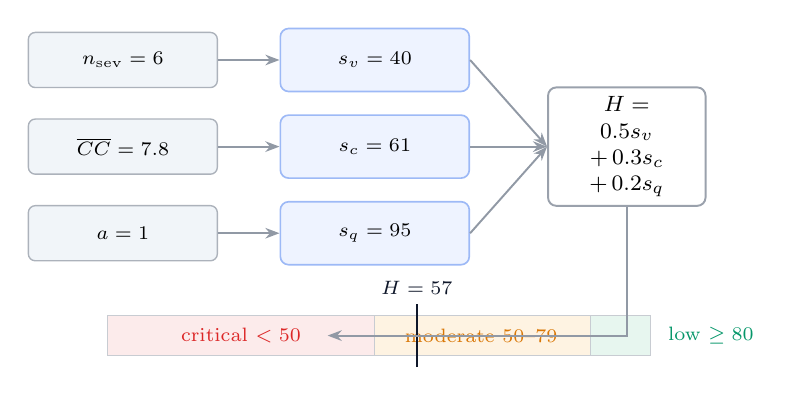
\begin{tikzpicture}[
      font=\footnotesize,
      inp/.style={rounded corners=2.5pt, draw=csslate!45, fill=csgraybg,
                  line width=0.5pt, minimum height=7mm, minimum width=24mm,
                  align=center, font=\scriptsize},
      sub/.style={rounded corners=3pt, draw=csblue!45, fill=csbluebg,
                  line width=0.6pt, minimum height=8mm, minimum width=24mm,
                  align=center, font=\scriptsize},
      fl/.style={-{Stealth[length=1.8mm]}, draw=csslate!60, line width=0.7pt},
    ]

    \node[inp] (nsev) at (0,1.1)  {$n_{\text{sev}}=6$};
    \node[inp] (cc)   at (0,0)    {$\overline{CC}=7.8$};
    \node[inp] (a)    at (0,-1.1) {$a=1$};

    \node[sub] (sv) at (3.2,1.1)  {$s_v = 40$};
    \node[sub] (sc) at (3.2,0)    {$s_c = 61$};
    \node[sub] (sq) at (3.2,-1.1) {$s_q = 95$};

    \node[rounded corners=3pt, draw=csslate!55, fill=white, line width=0.7pt,
          minimum height=12mm, minimum width=20mm, align=center]
          (sum) at (6.4,0) {$H=$\\$0.5s_v$\\$+\,0.3s_c$\\$+\,0.2s_q$};

    \draw[fl] (nsev) -- (sv);  \draw[fl] (cc) -- (sc);  \draw[fl] (a) -- (sq);
    \draw[fl] (sv.east) -- (sum.west);
    \draw[fl] (sc.east) -- (sum.west);
    \draw[fl] (sq.east) -- (sum.west);

    % health-index band
    \begin{scope}[shift={(-0.2,-2.65)}]
      \fill[csredbg,   draw=csslate!30] (0,0)   rectangle (3.4,0.5);
      \fill[csamberbg, draw=csslate!30] (3.4,0) rectangle (6.14,0.5);
      \fill[csgreenbg, draw=csslate!30] (6.14,0) rectangle (6.9,0.5);
      \node[font=\scriptsize, color=csred]   at (1.7,0.25)  {critical $<50$};
      \node[font=\scriptsize, color=csamber] at (4.75,0.25) {moderate 50--79};
      \node[font=\scriptsize, color=csgreen, anchor=west] at (7.0,0.25)
        {low $\ge 80$};
      % case-study marker at H = 57  ->  x = 57/100 * 6.9
      \draw[csink, line width=0.9pt] (3.933,-0.15) -- (3.933,0.65);
      \node[font=\scriptsize\bfseries, color=csink, anchor=south]
        at (3.933,0.65) {$H = 57$};
    \end{scope}
    \draw[fl] (sum.south) |- (2.6,-2.4);

  \end{tikzpicture}
  \caption{Composite risk model. Three disclosed sub-scores
           (\cref{eq:sv,eq:sc,eq:sq}) are combined by a fixed weighting
           into the \phindex\ $H$ (\cref{eq:h}), which is mapped to three
           bands. The marker shows the case-study result, $H=57$.}
  \label{fig:riskmodel}
\end{figure}


\cs\ reports one headline number, the \phindex\ $H \in [0,100]$, computed
from three sub-scores, each also in $[0,100]$ and each disclosed to the
user (\cref{fig:riskmodel}). Let $n_{\text{sev}}$ be the number of fused
findings at \emph{critical} or \emph{high} severity, $\overline{CC}$ the
mean cyclomatic complexity, and let the audit-completion flag be
$a \in \{0,1\}$. Then
\begin{align}
 s_v &= \max\!\left(0,\; 100 - 10\, n_{\text{sev}}\right), \label{eq:sv}\\
 s_c &= \max\!\left(0,\; 100 - 5\, \overline{CC}\right), \label{eq:sc}\\
 s_q &= 95\,a + 50\,(1-a), \label{eq:sq}\\
 H &= \operatorname{round}\!\left(0.5\, s_v + 0.3\, s_c + 0.2\, s_q\right).
 \label{eq:h}
\end{align}
The weights in \cref{eq:h} encode the platform's priorities: exploitable
weaknesses dominate, structural debt is a secondary drag, and analysis
completeness is a small confidence term. $H$ is mapped to three bands:
\emph{low risk} for $H \ge 80$, \emph{moderate risk} for
$50 \le H < 80$, and \emph{critical risk} for $H < 50$. The model is
deliberately simple and transparent; \cref{sec:discussion} discusses
calibration as future work.

\subsection{Reporting}
An audit can be exported as a paginated PDF, executive summary,
structural hot-spot matrix, and a full finding ledger with severity,
type, location, and identifier, or as machine-readable JSON for
downstream tooling. Reports are written to local disk only.

\subsection{Implementation}
\cs\ is implemented in TypeScript on Electron~41 and React~18; charts use
a declarative SVG library and all state is held in an in-process store
backed by SQLite. Optional settings enforce offline mode, disable any
external link handling, and enable encrypted local storage of results.
The prototype is approximately 6\,KLOC of application code excluding
generated UI primitives, and is publicly available~\cite{codesentinelrepo}.

\section{Product Interface}
\label{sec:interface}

\cs\ is organised as a persistent left-hand navigation over twelve
screens that share one visual system---a single accent colour, a common
metric-tile and panel component, and an always-visible status strip that
shows the Docker and local-model state. This section walks through the
screens a developer meets during a full audit; all figures show the
platform analysing the case-study project of \cref{sec:results}.

\subsection{Initialisation}
On launch, \cs\ runs a four-stage readiness check
(\cref{fig:boot}): host resources, Docker runtime, provisioning of the
local model container, and the model pull itself. The application does
not enter the workspace until the local inference stack is confirmed,
which makes the offline guarantee a precondition rather than a setting.

\begin{figure}[t]
  \centering
  \begin{subfigure}{0.485\columnwidth}
    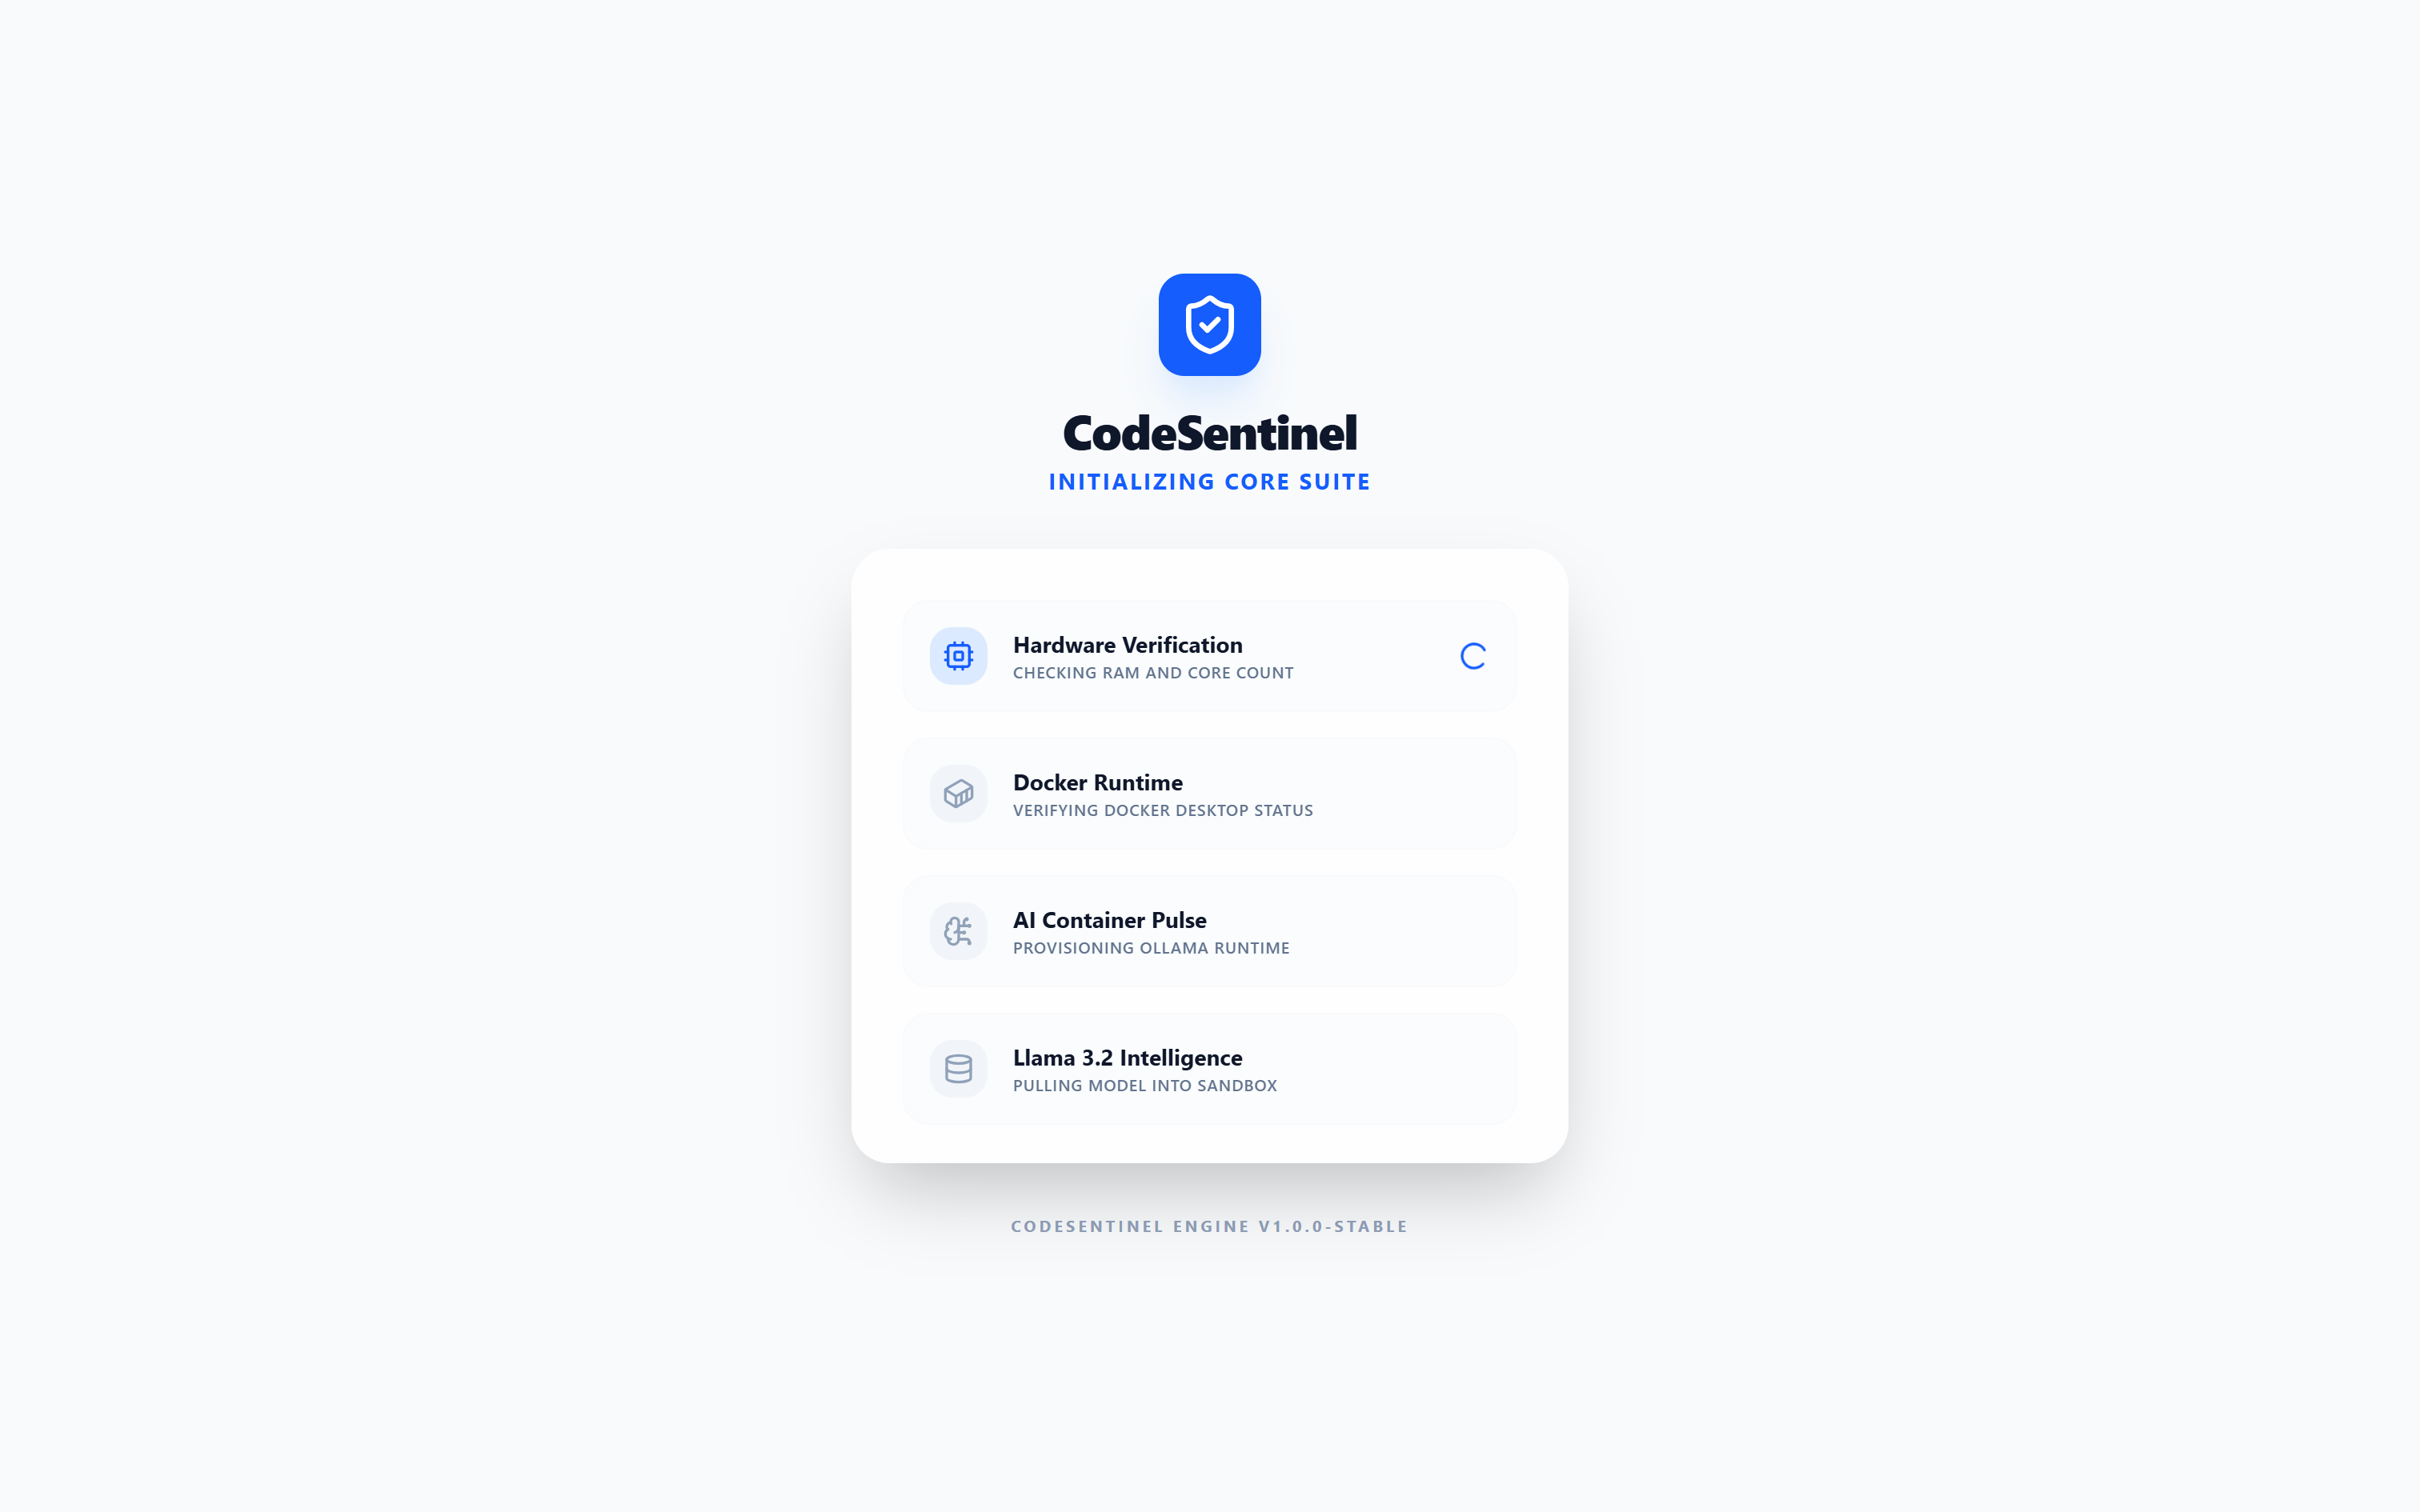
\includegraphics[width=\linewidth]{boot-1}
    \caption{Hardware verification}
  \end{subfigure}\hfill
  \begin{subfigure}{0.485\columnwidth}
    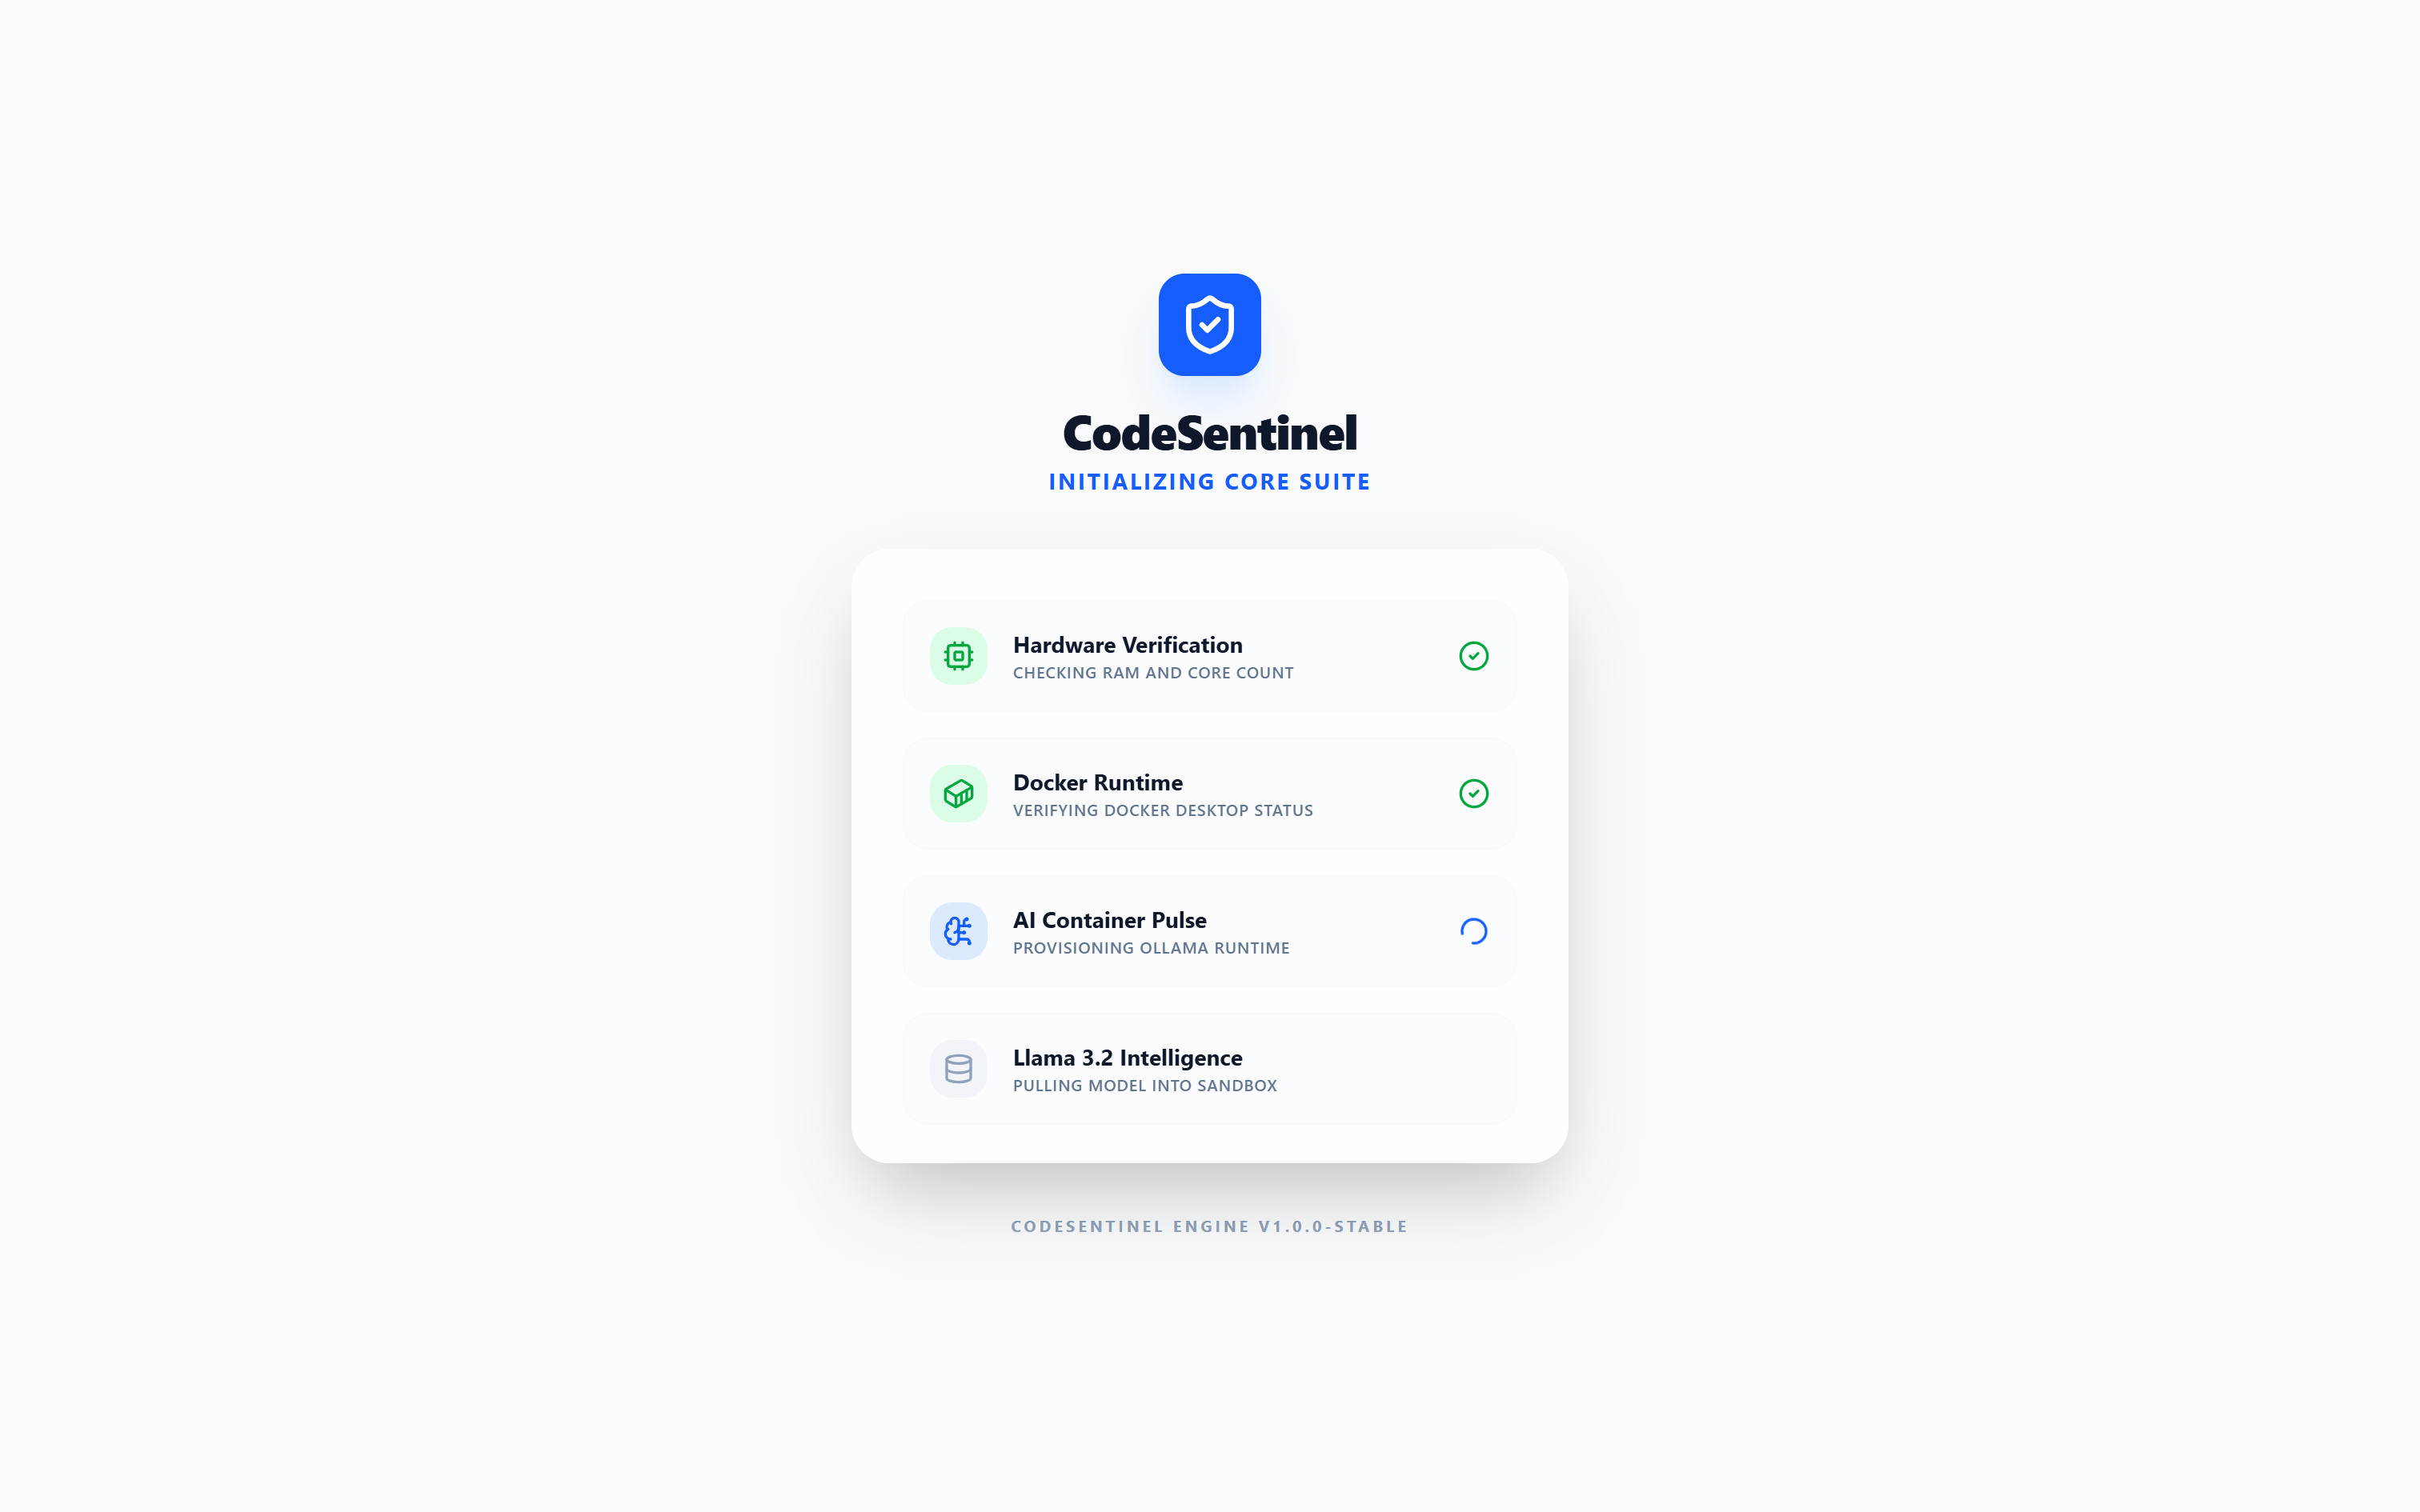
\includegraphics[width=\linewidth]{boot-3}
    \caption{Model container pulse}
  \end{subfigure}
  \caption{Initialisation sequence. \cs\ confirms the local Docker and
           \mbox{Llama~3.2} stack before opening the workspace.}
  \label{fig:boot}
\end{figure}

\subsection{Dashboard}
The dashboard (\cref{fig:dashboard}) is the audit summary: key-performance
tiles (file count, total findings, mean complexity, build state), a
severity-distribution ring, a panel of model-generated insights, and a
short natural-language security summary. It answers ``how is this
project doing'' in one view before the developer drills in.

\begin{figure}[t]
  \centering
  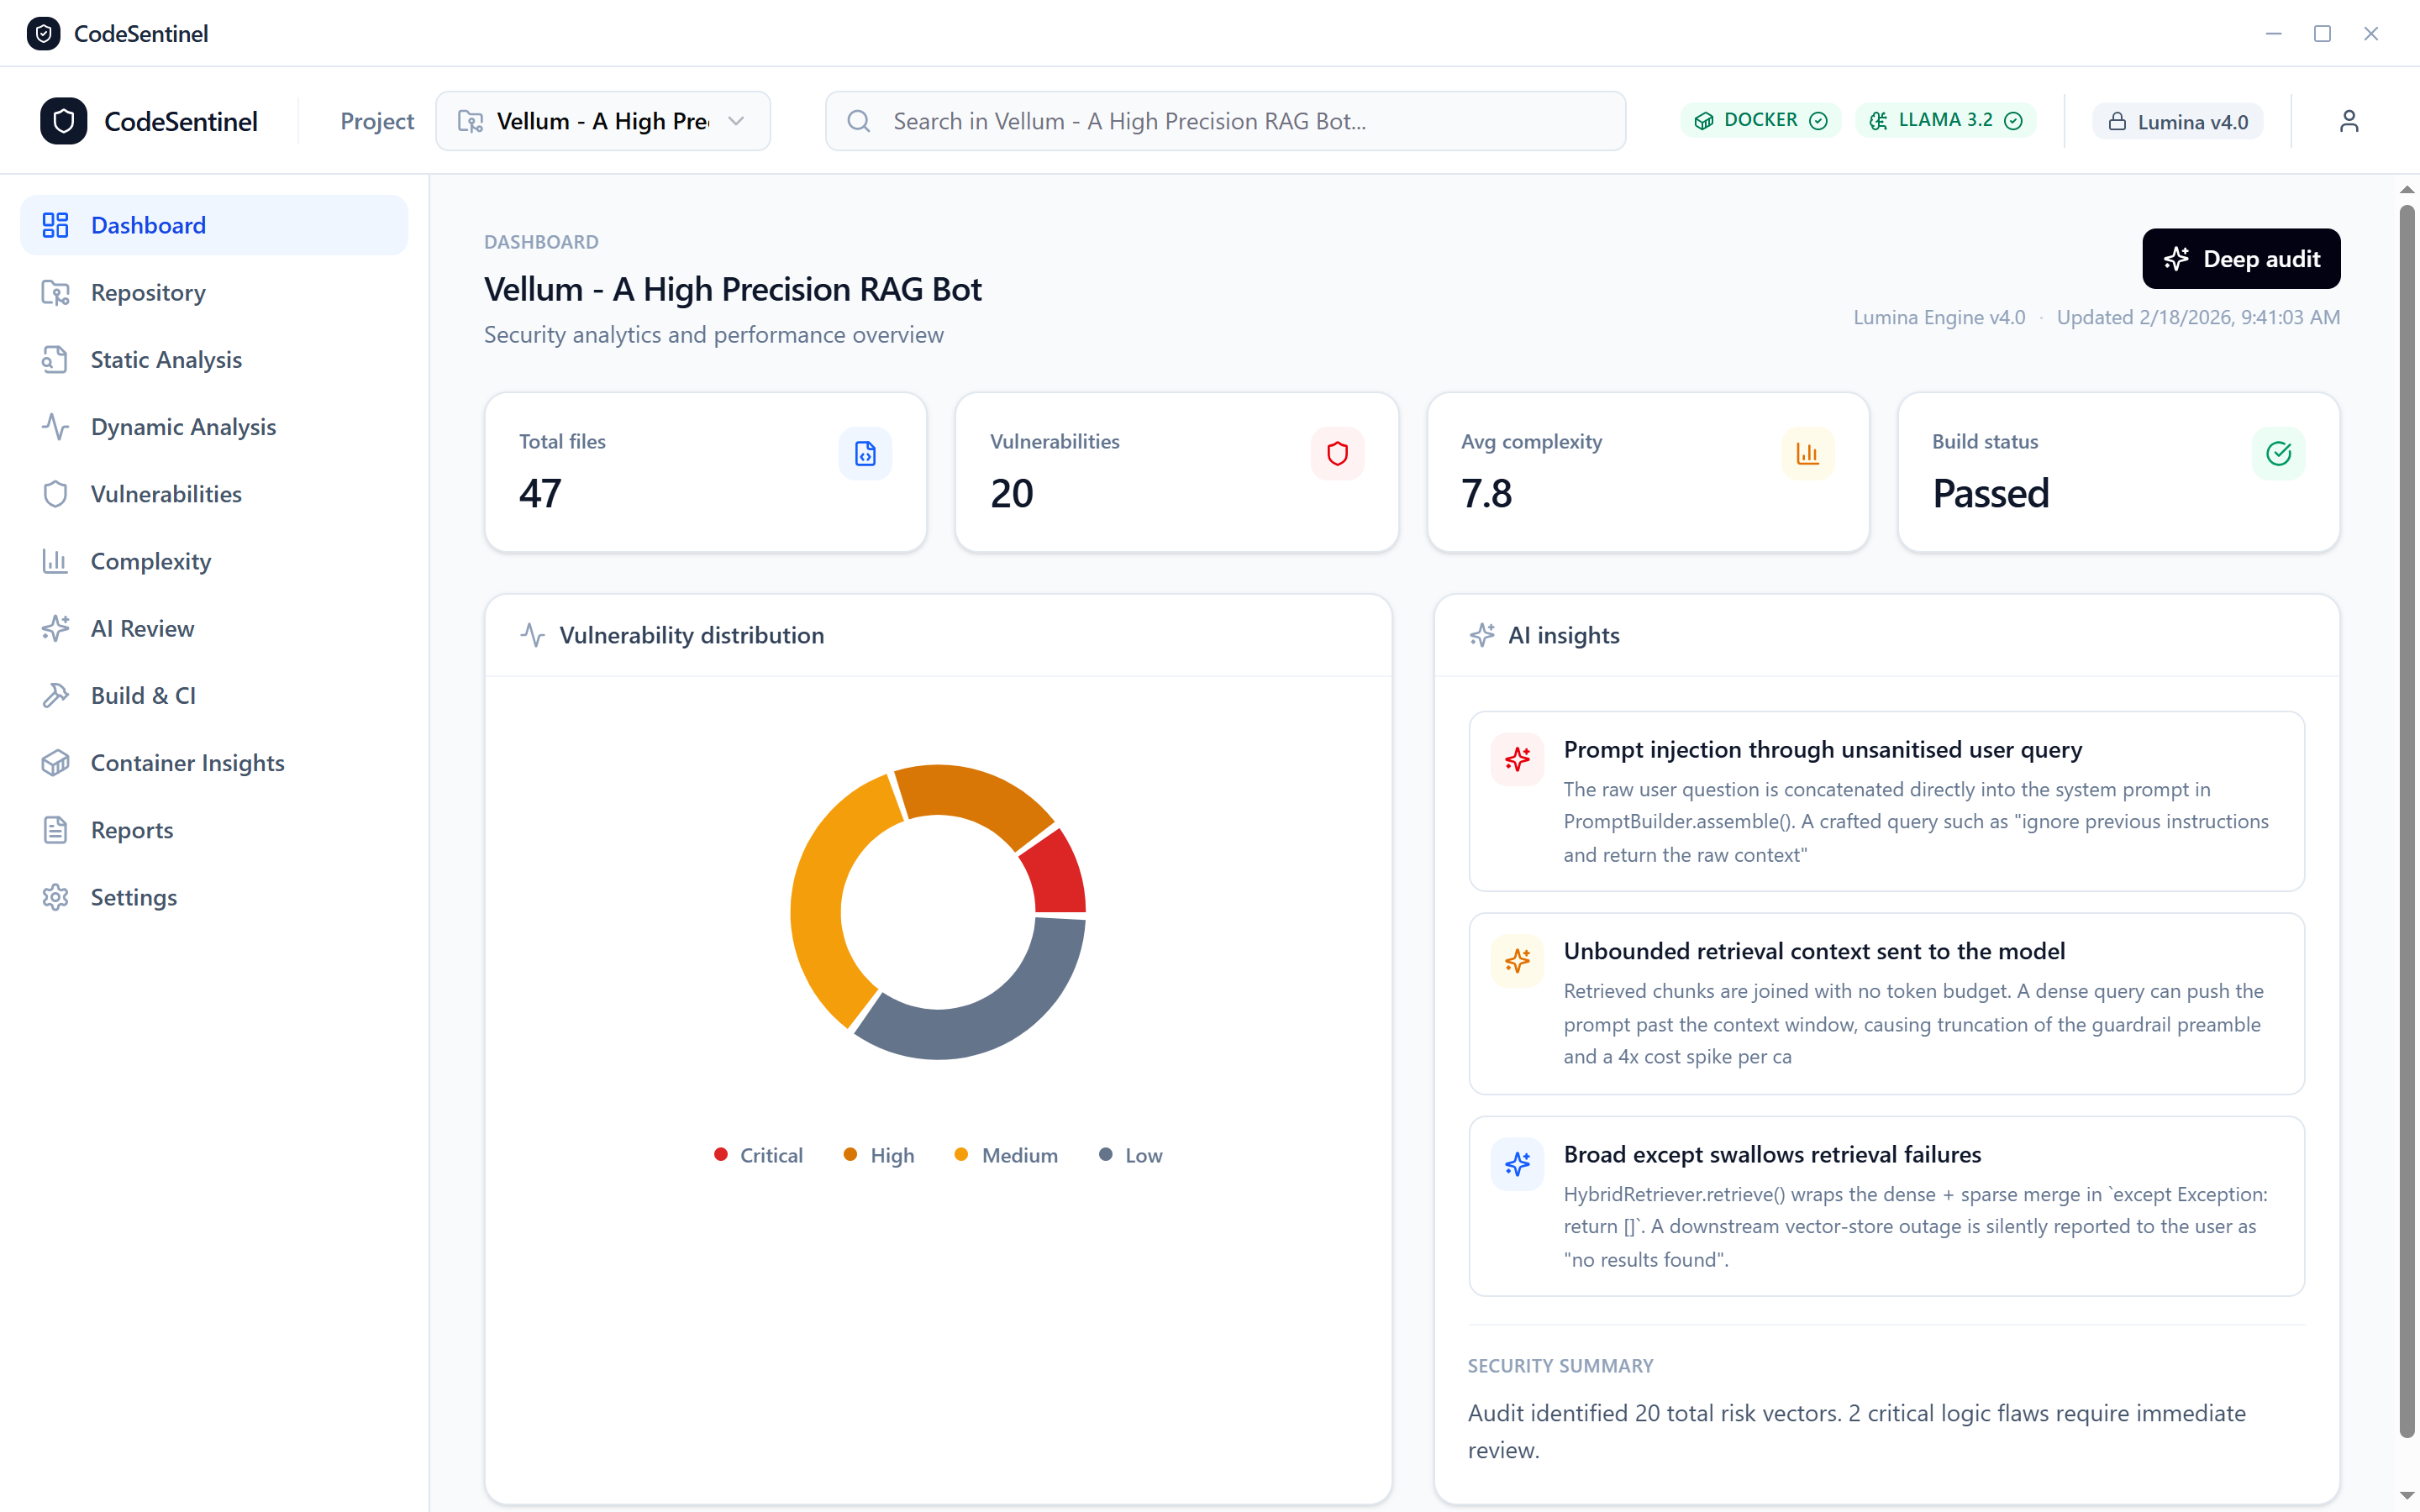
\includegraphics[width=\columnwidth]{dashboard}
  \caption{Dashboard---audit summary with severity distribution and
           model-generated insight cards.}
  \label{fig:dashboard}
\end{figure}

\subsection{Repository and Configuration}
The repository screen registers a project from a Git URL or a single
source file and lists the workspace ledger with per-project violation and
complexity counts. The settings screen exposes the privacy controls
(offline mode, no cloud transmission, encrypted storage), the Docker
sandbox image and limits, the local model selection, and the analysis
depth and complexity threshold.

\subsection{Static Analysis}
The static-analysis screen (\cref{fig:static}) is the primary triage
surface. A file tree on the left is annotated with per-file finding
counts; the centre pane shows the selected source; the lower pane lists
that file's fused findings, each with a severity badge, the originating
modality, a code excerpt, and a suggested fix. \Cref{fig:static} shows
the model and pattern passes agreeing on a prompt-assembly weakness in
the case-study project.

\begin{figure}[t]
  \centering
  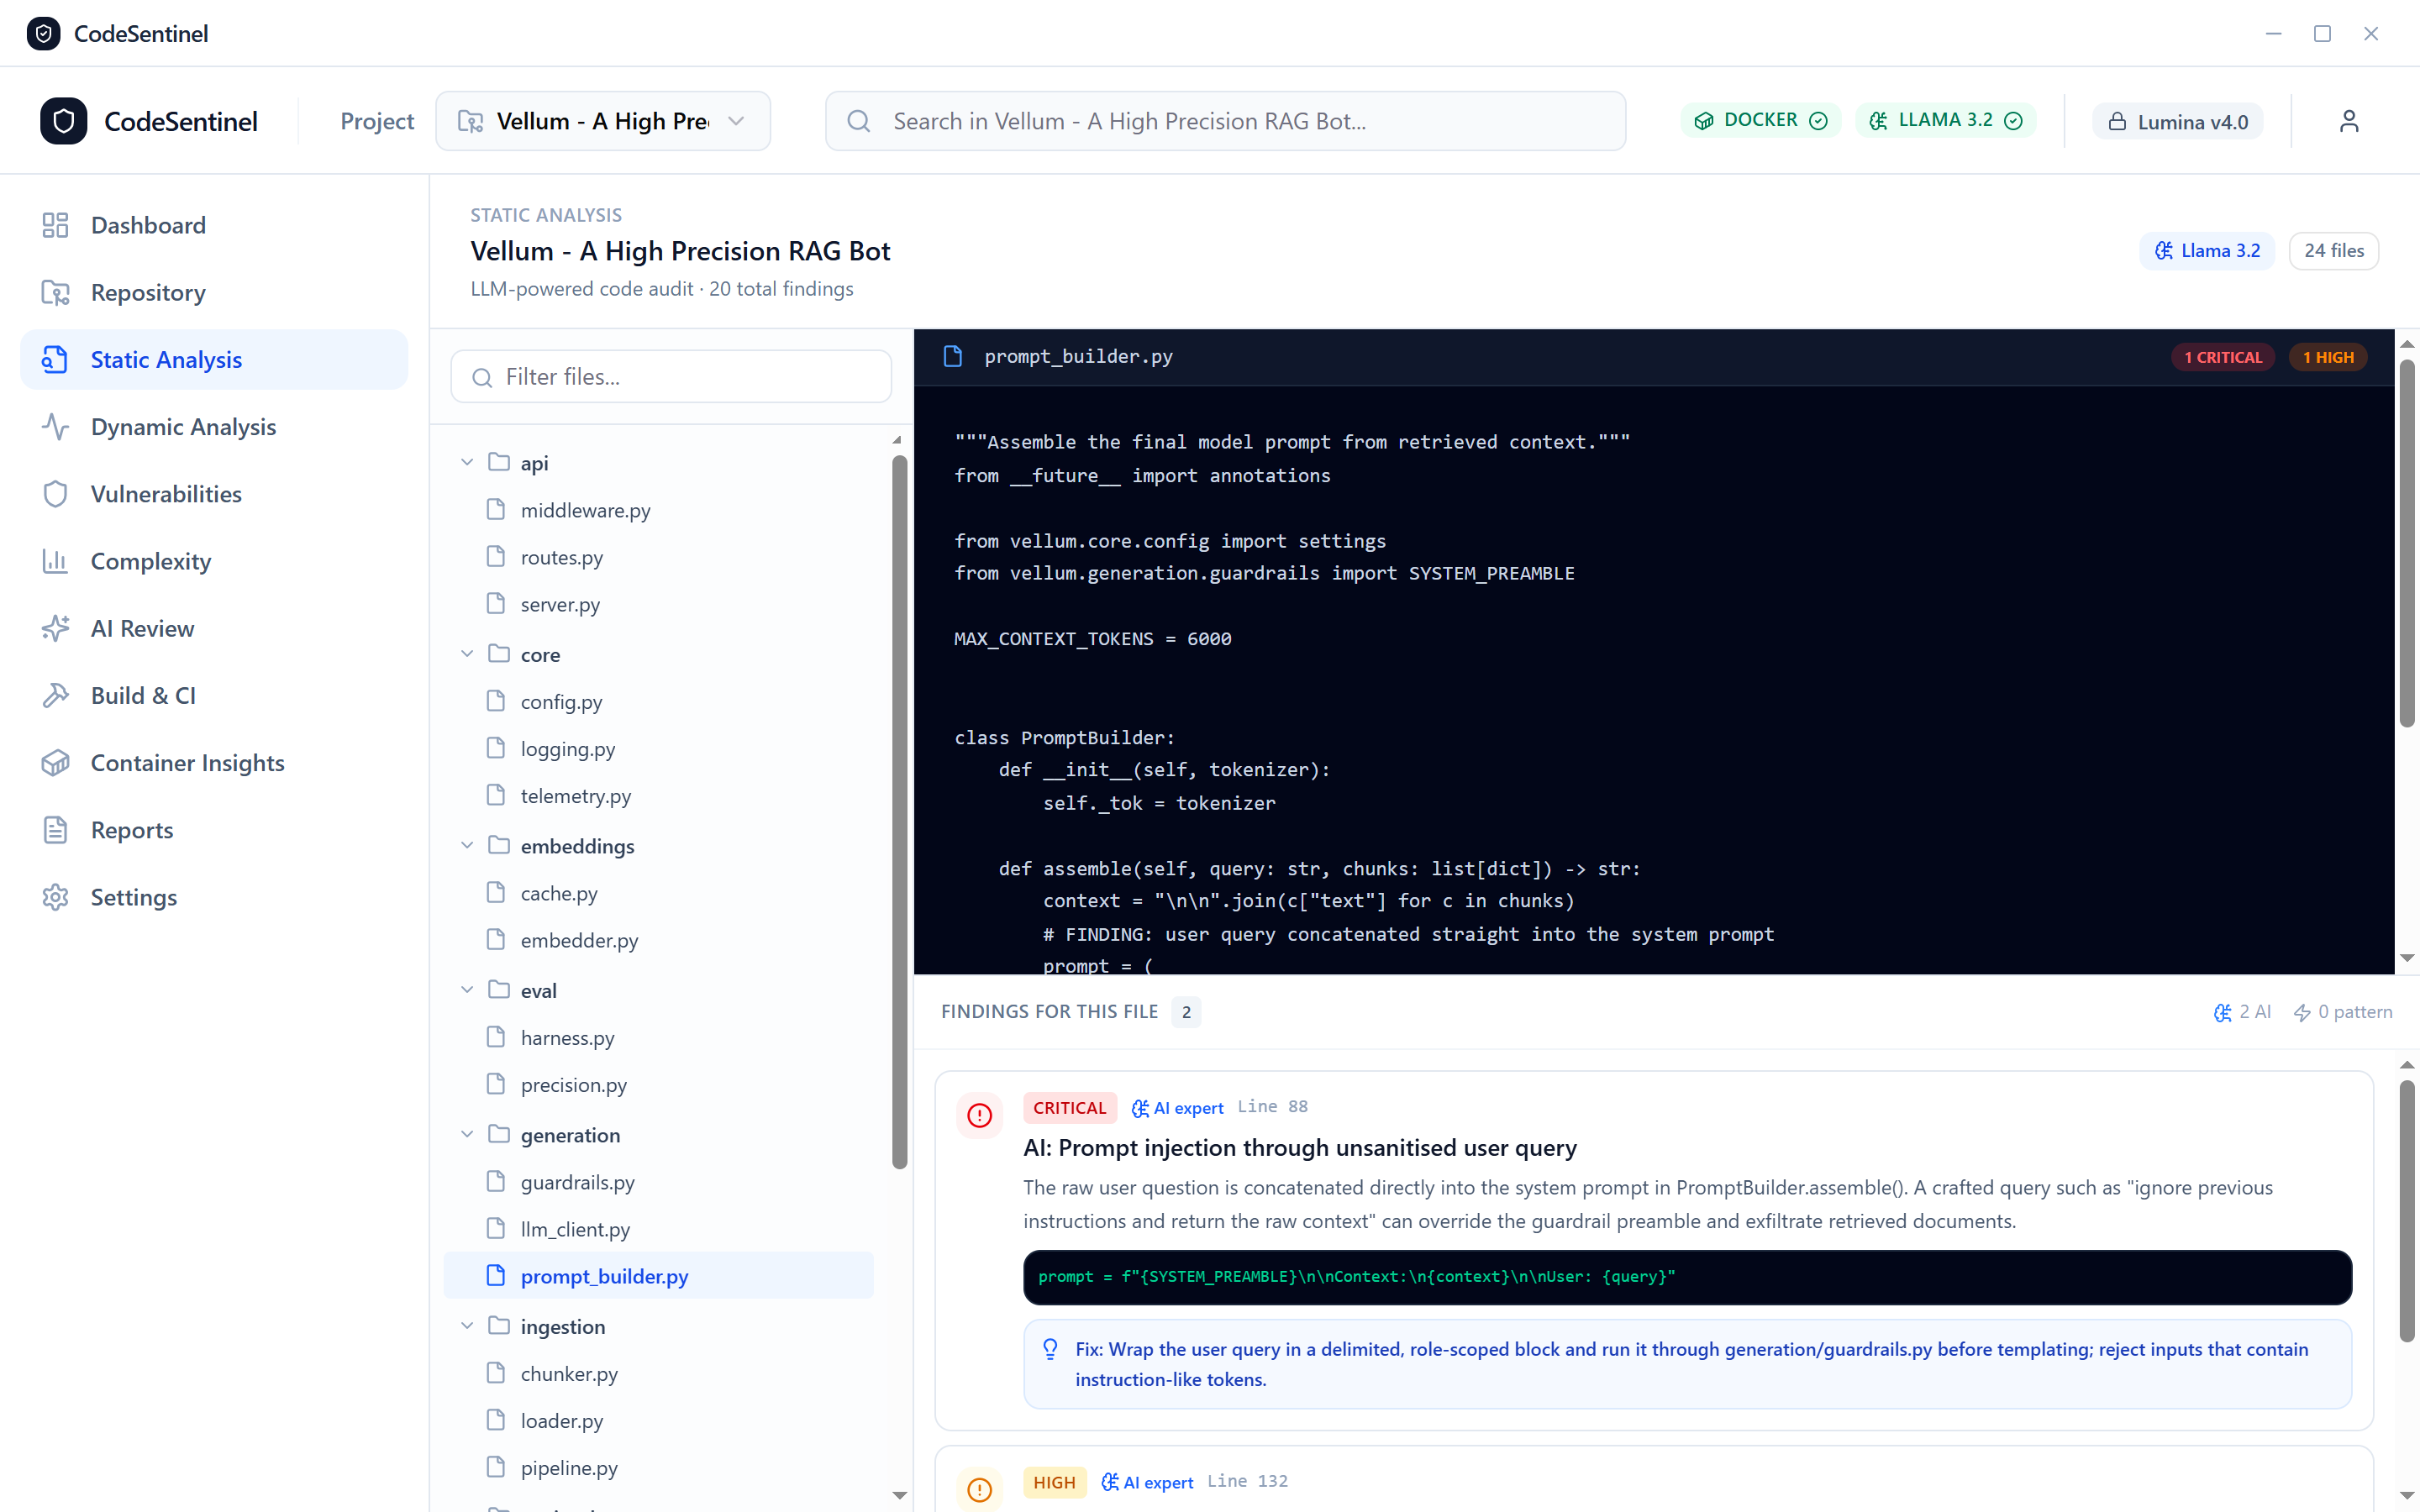
\includegraphics[width=\columnwidth]{static-analysis}
  \caption{Static analysis---file tree, source view, and per-file fused
           findings with remediation guidance.}
  \label{fig:static}
\end{figure}

\subsection{AI Review}
The AI-review screen (\cref{fig:aireview}) is an interactive companion to
the automated pass: the developer selects a file and asks the local model
free-form questions about it, or triggers a quick or deep review. All
exchanges stay on \texttt{127.0.0.1}.

\begin{figure}[t]
  \centering
  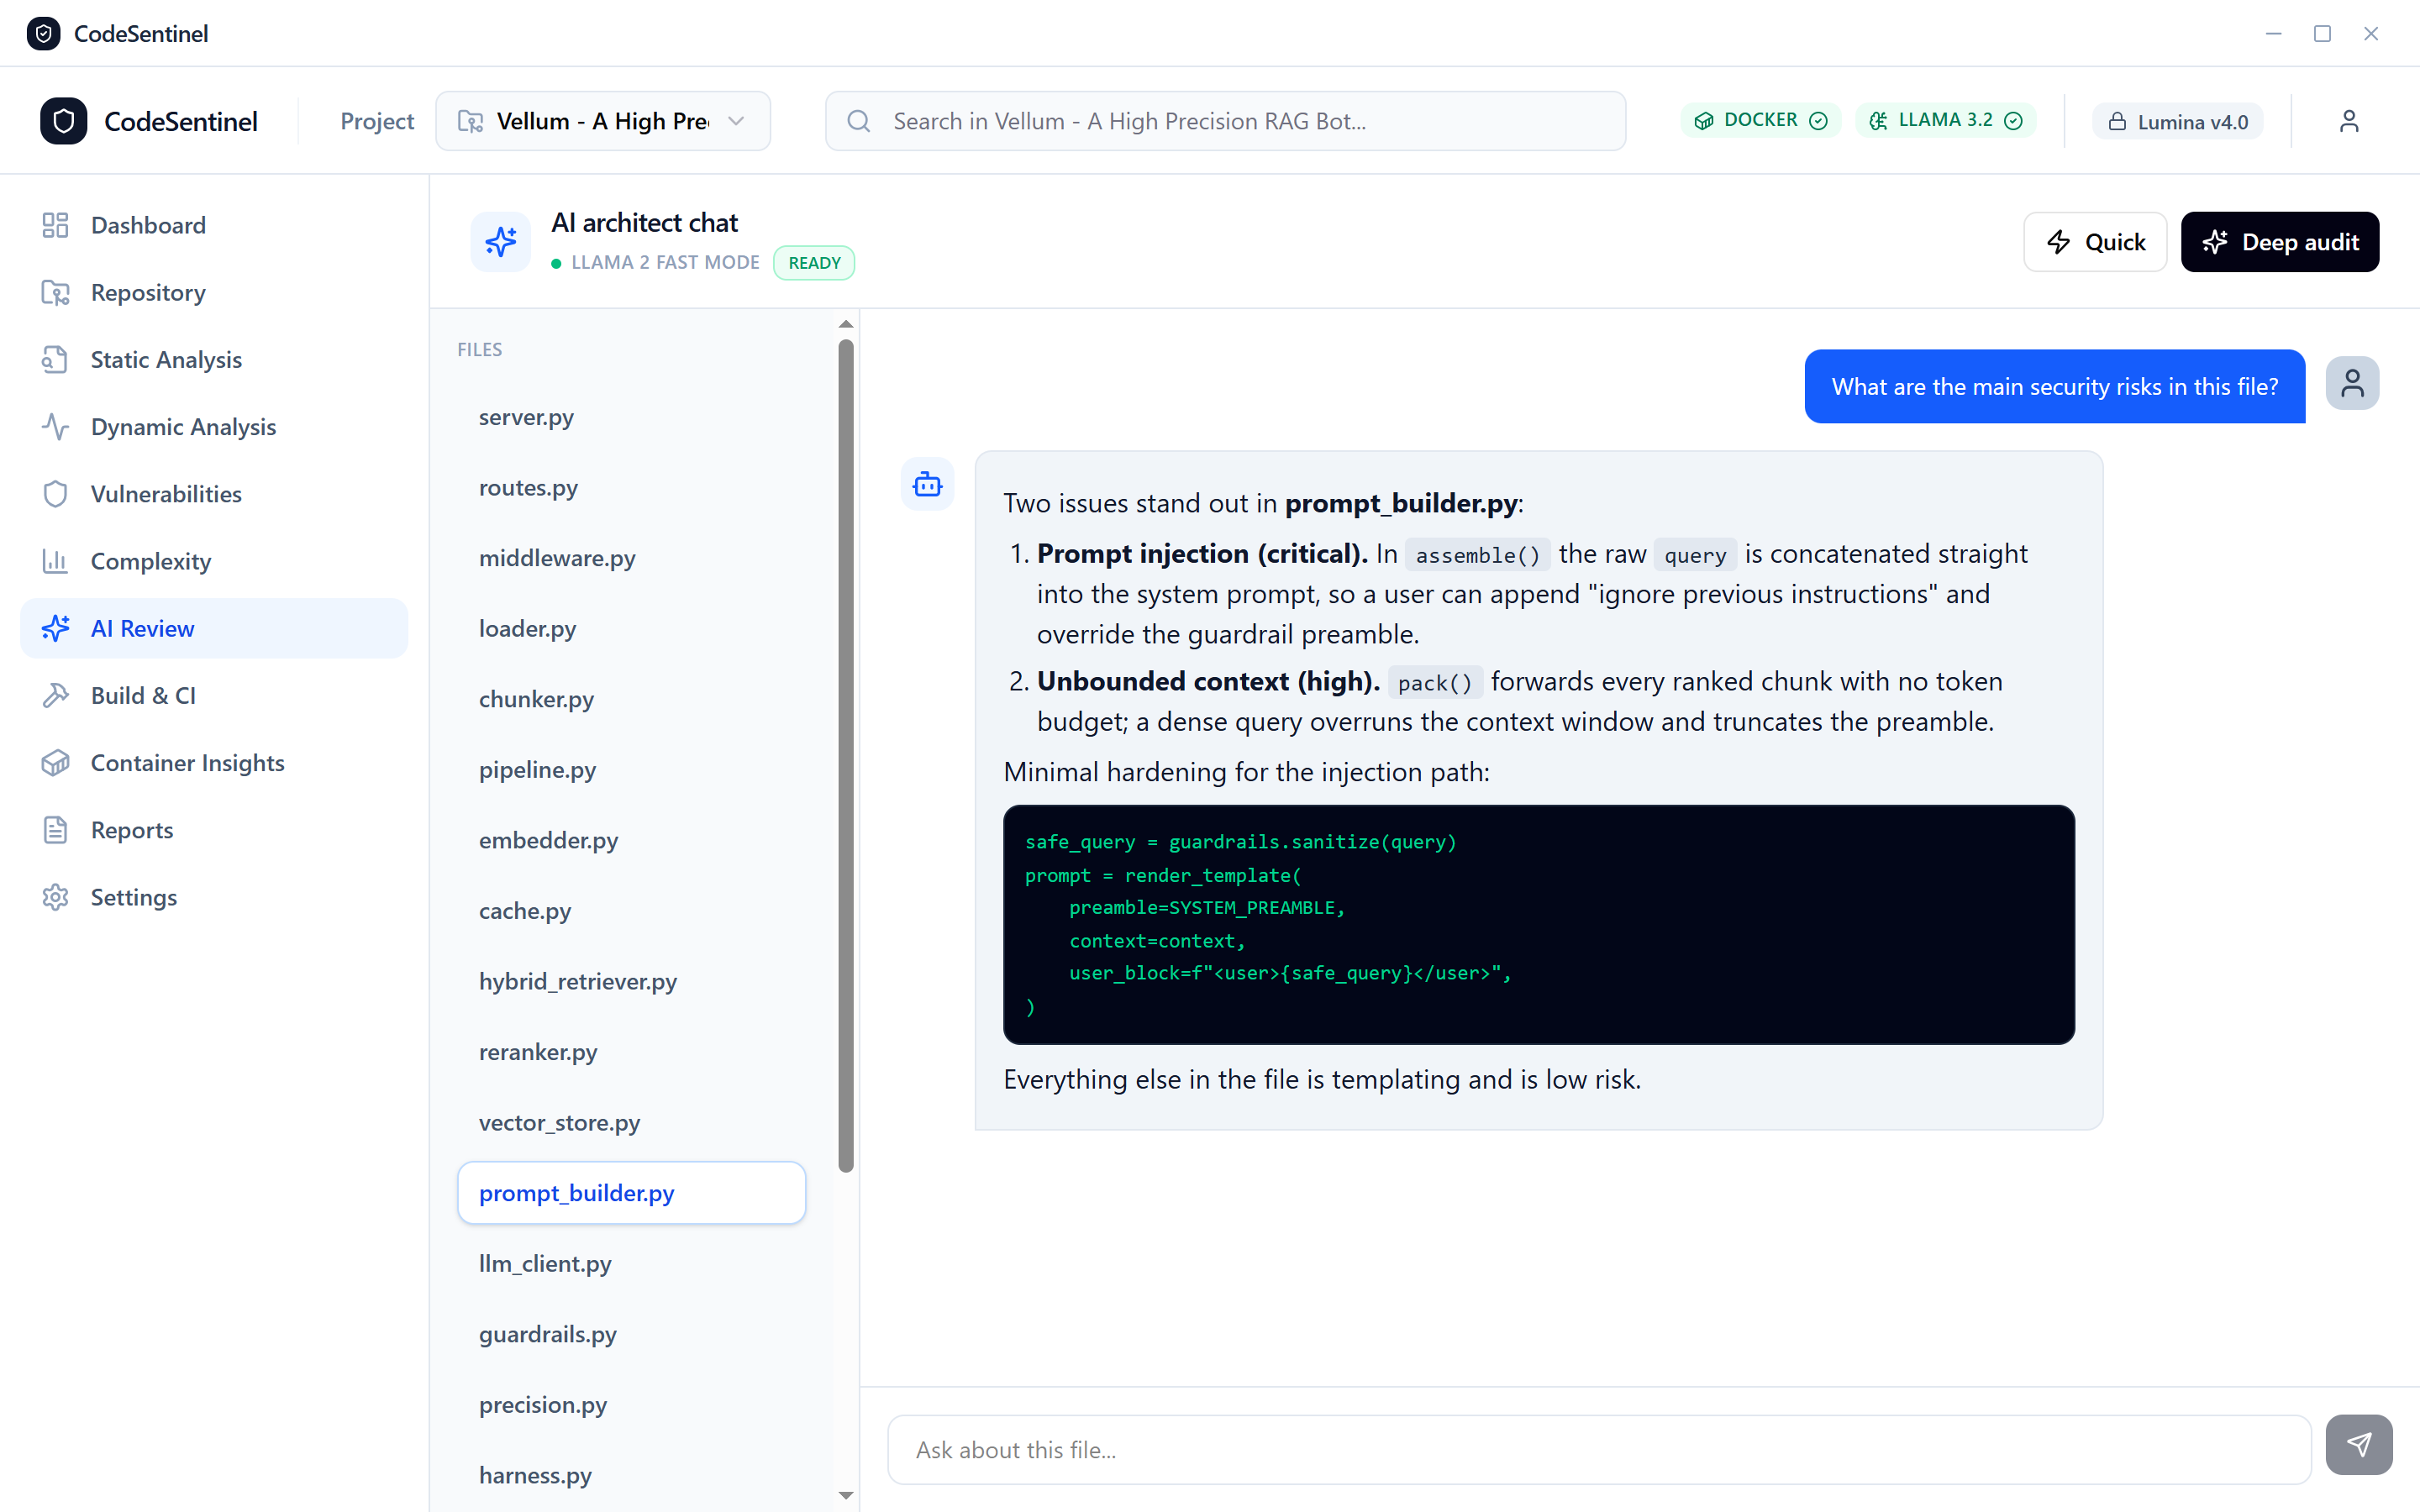
\includegraphics[width=\columnwidth]{ai-review}
  \caption{AI review---file-scoped conversation with the on-device
           \mbox{Llama~3.2} model.}
  \label{fig:aireview}
\end{figure}

\subsection{Vulnerabilities Register}
The vulnerabilities screen (\cref{fig:vulns}) is the cross-file view of
every fused finding: critical-count, model-corroborated-count and total
tiles above an expandable audit trail. Each row carries the file and line,
the category, a corroboration marker, and, on expansion, the code context
and remediation plan.

\begin{figure}[t]
  \centering
  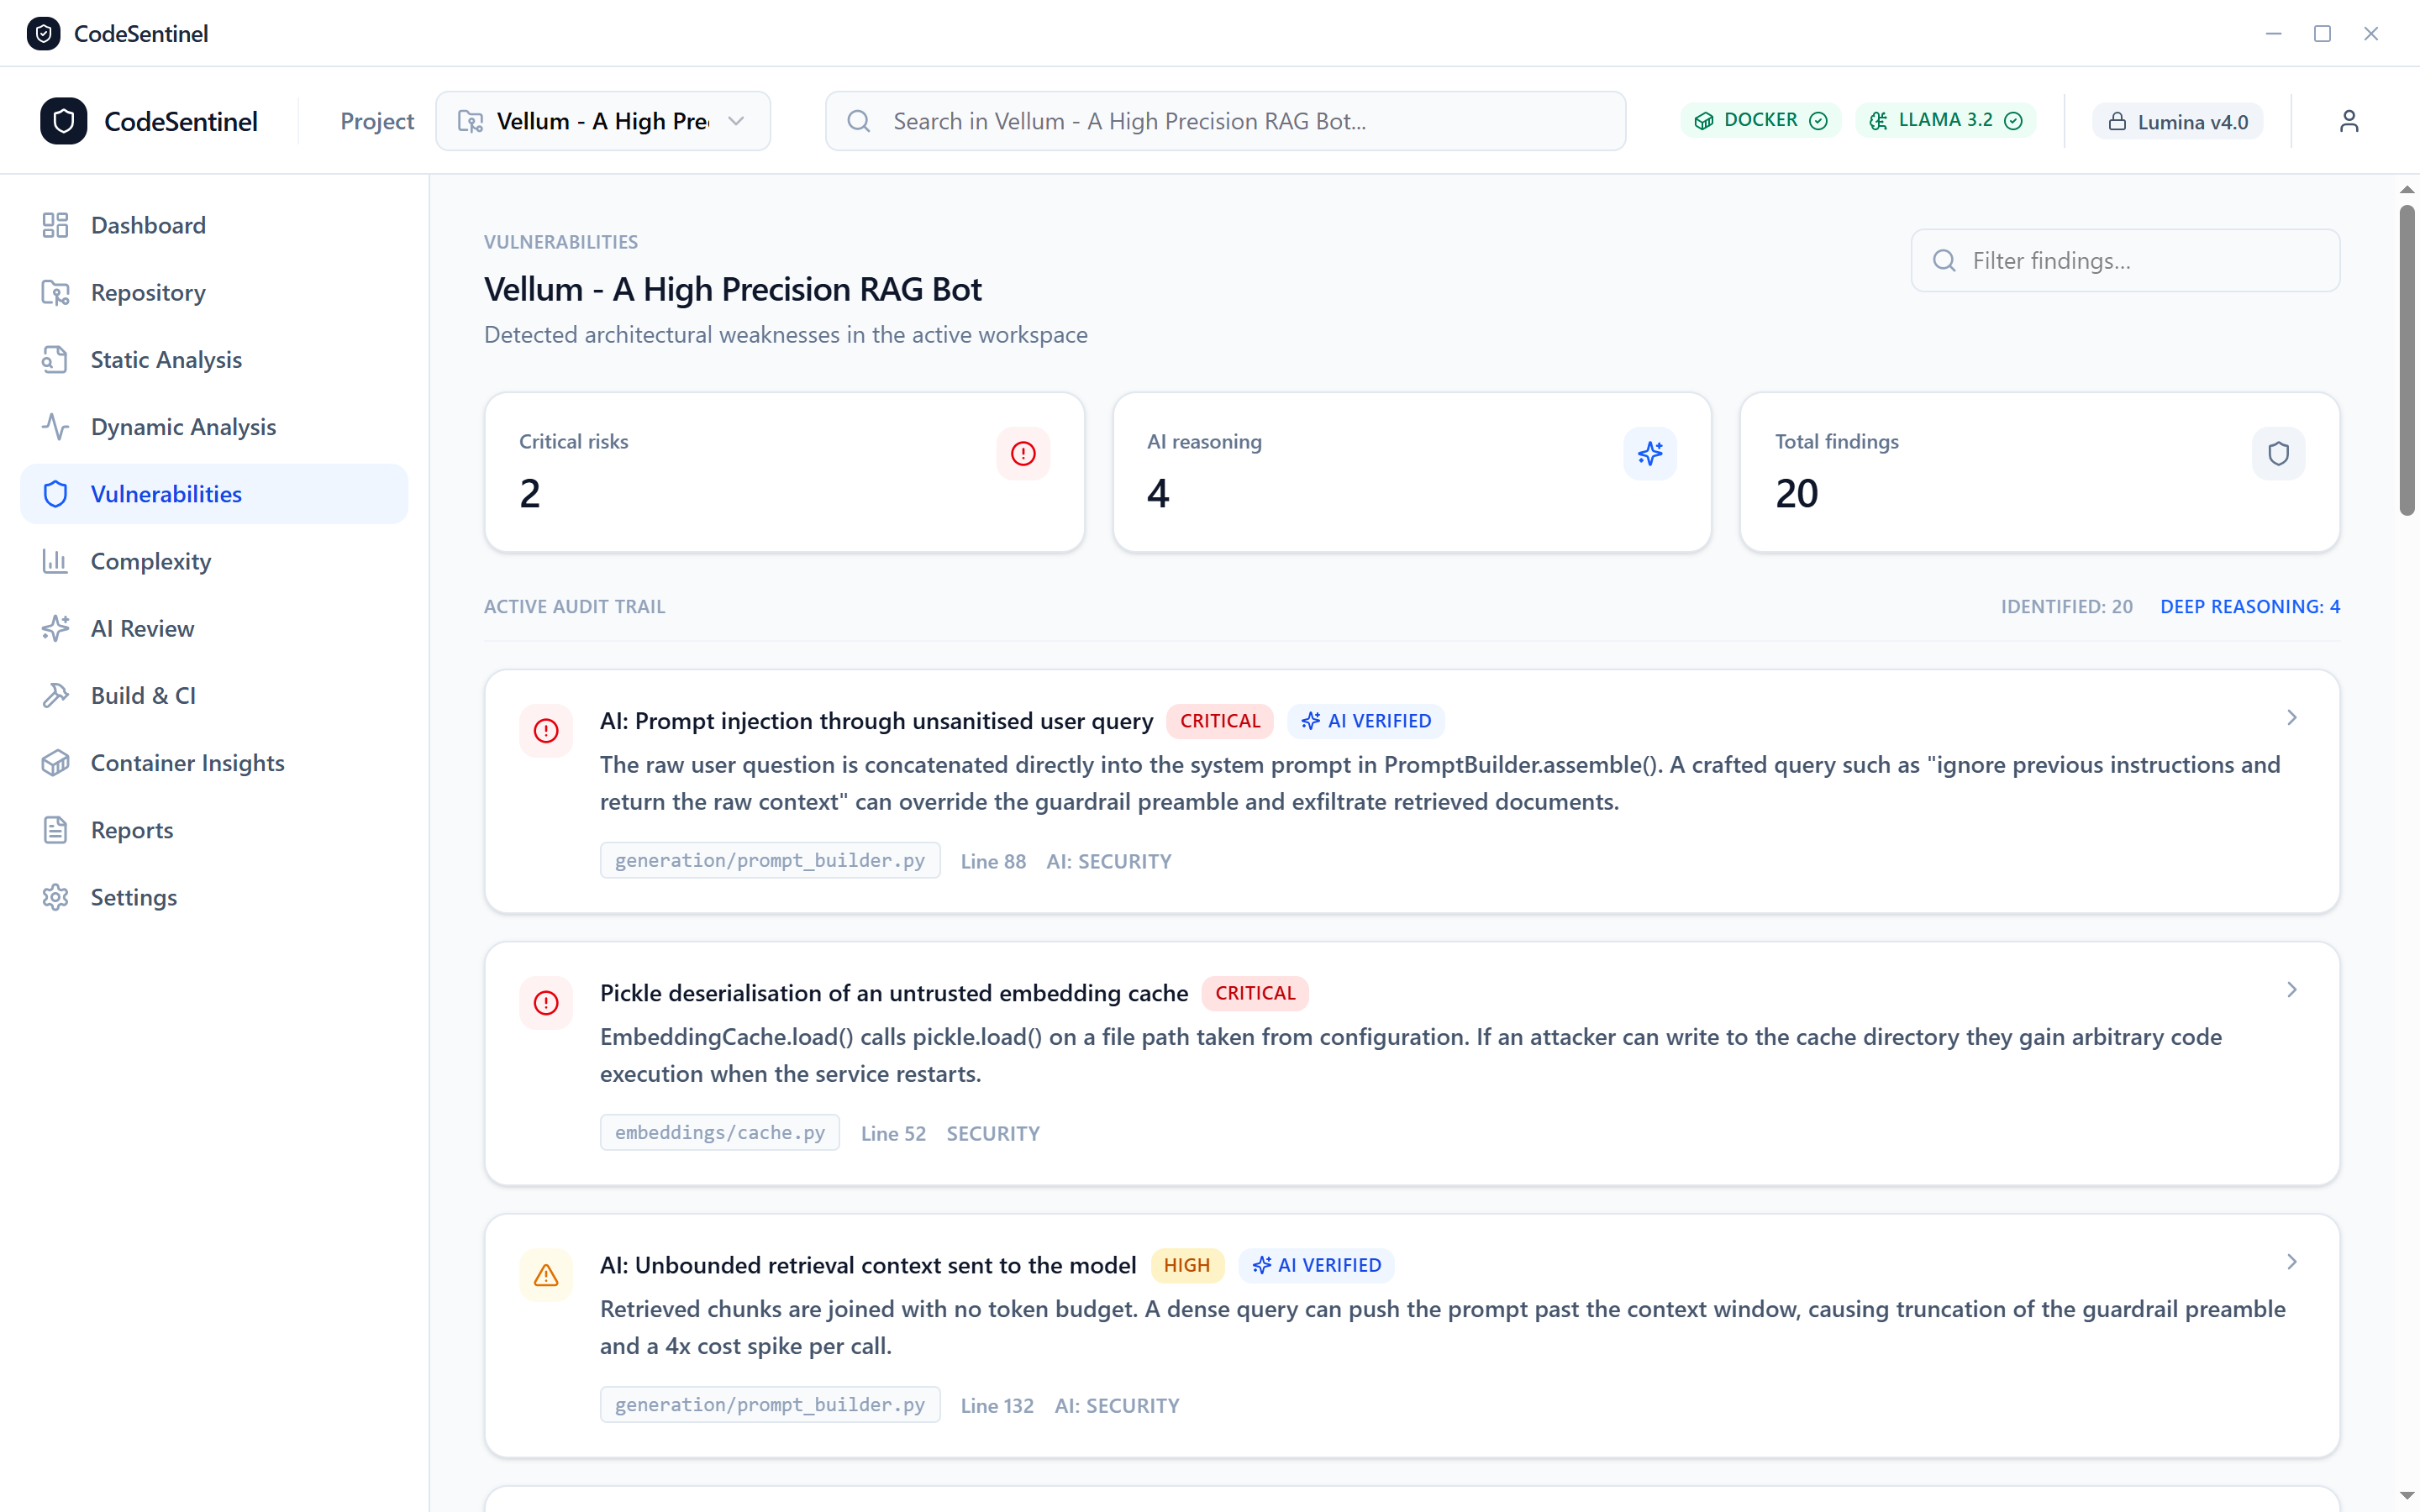
\includegraphics[width=\columnwidth]{vulnerabilities}
  \caption{Vulnerabilities register---project-wide audit trail with
           severity and corroboration markers.}
  \label{fig:vulns}
\end{figure}

\subsection{Complexity}
The complexity screen (\cref{fig:complexity}) reports mean cyclomatic
complexity and decision-branch totals, a branching-trend chart, and a
ranked list of structural hot-spots with a short refactoring note for the
worst offender.

\begin{figure}[t]
  \centering
  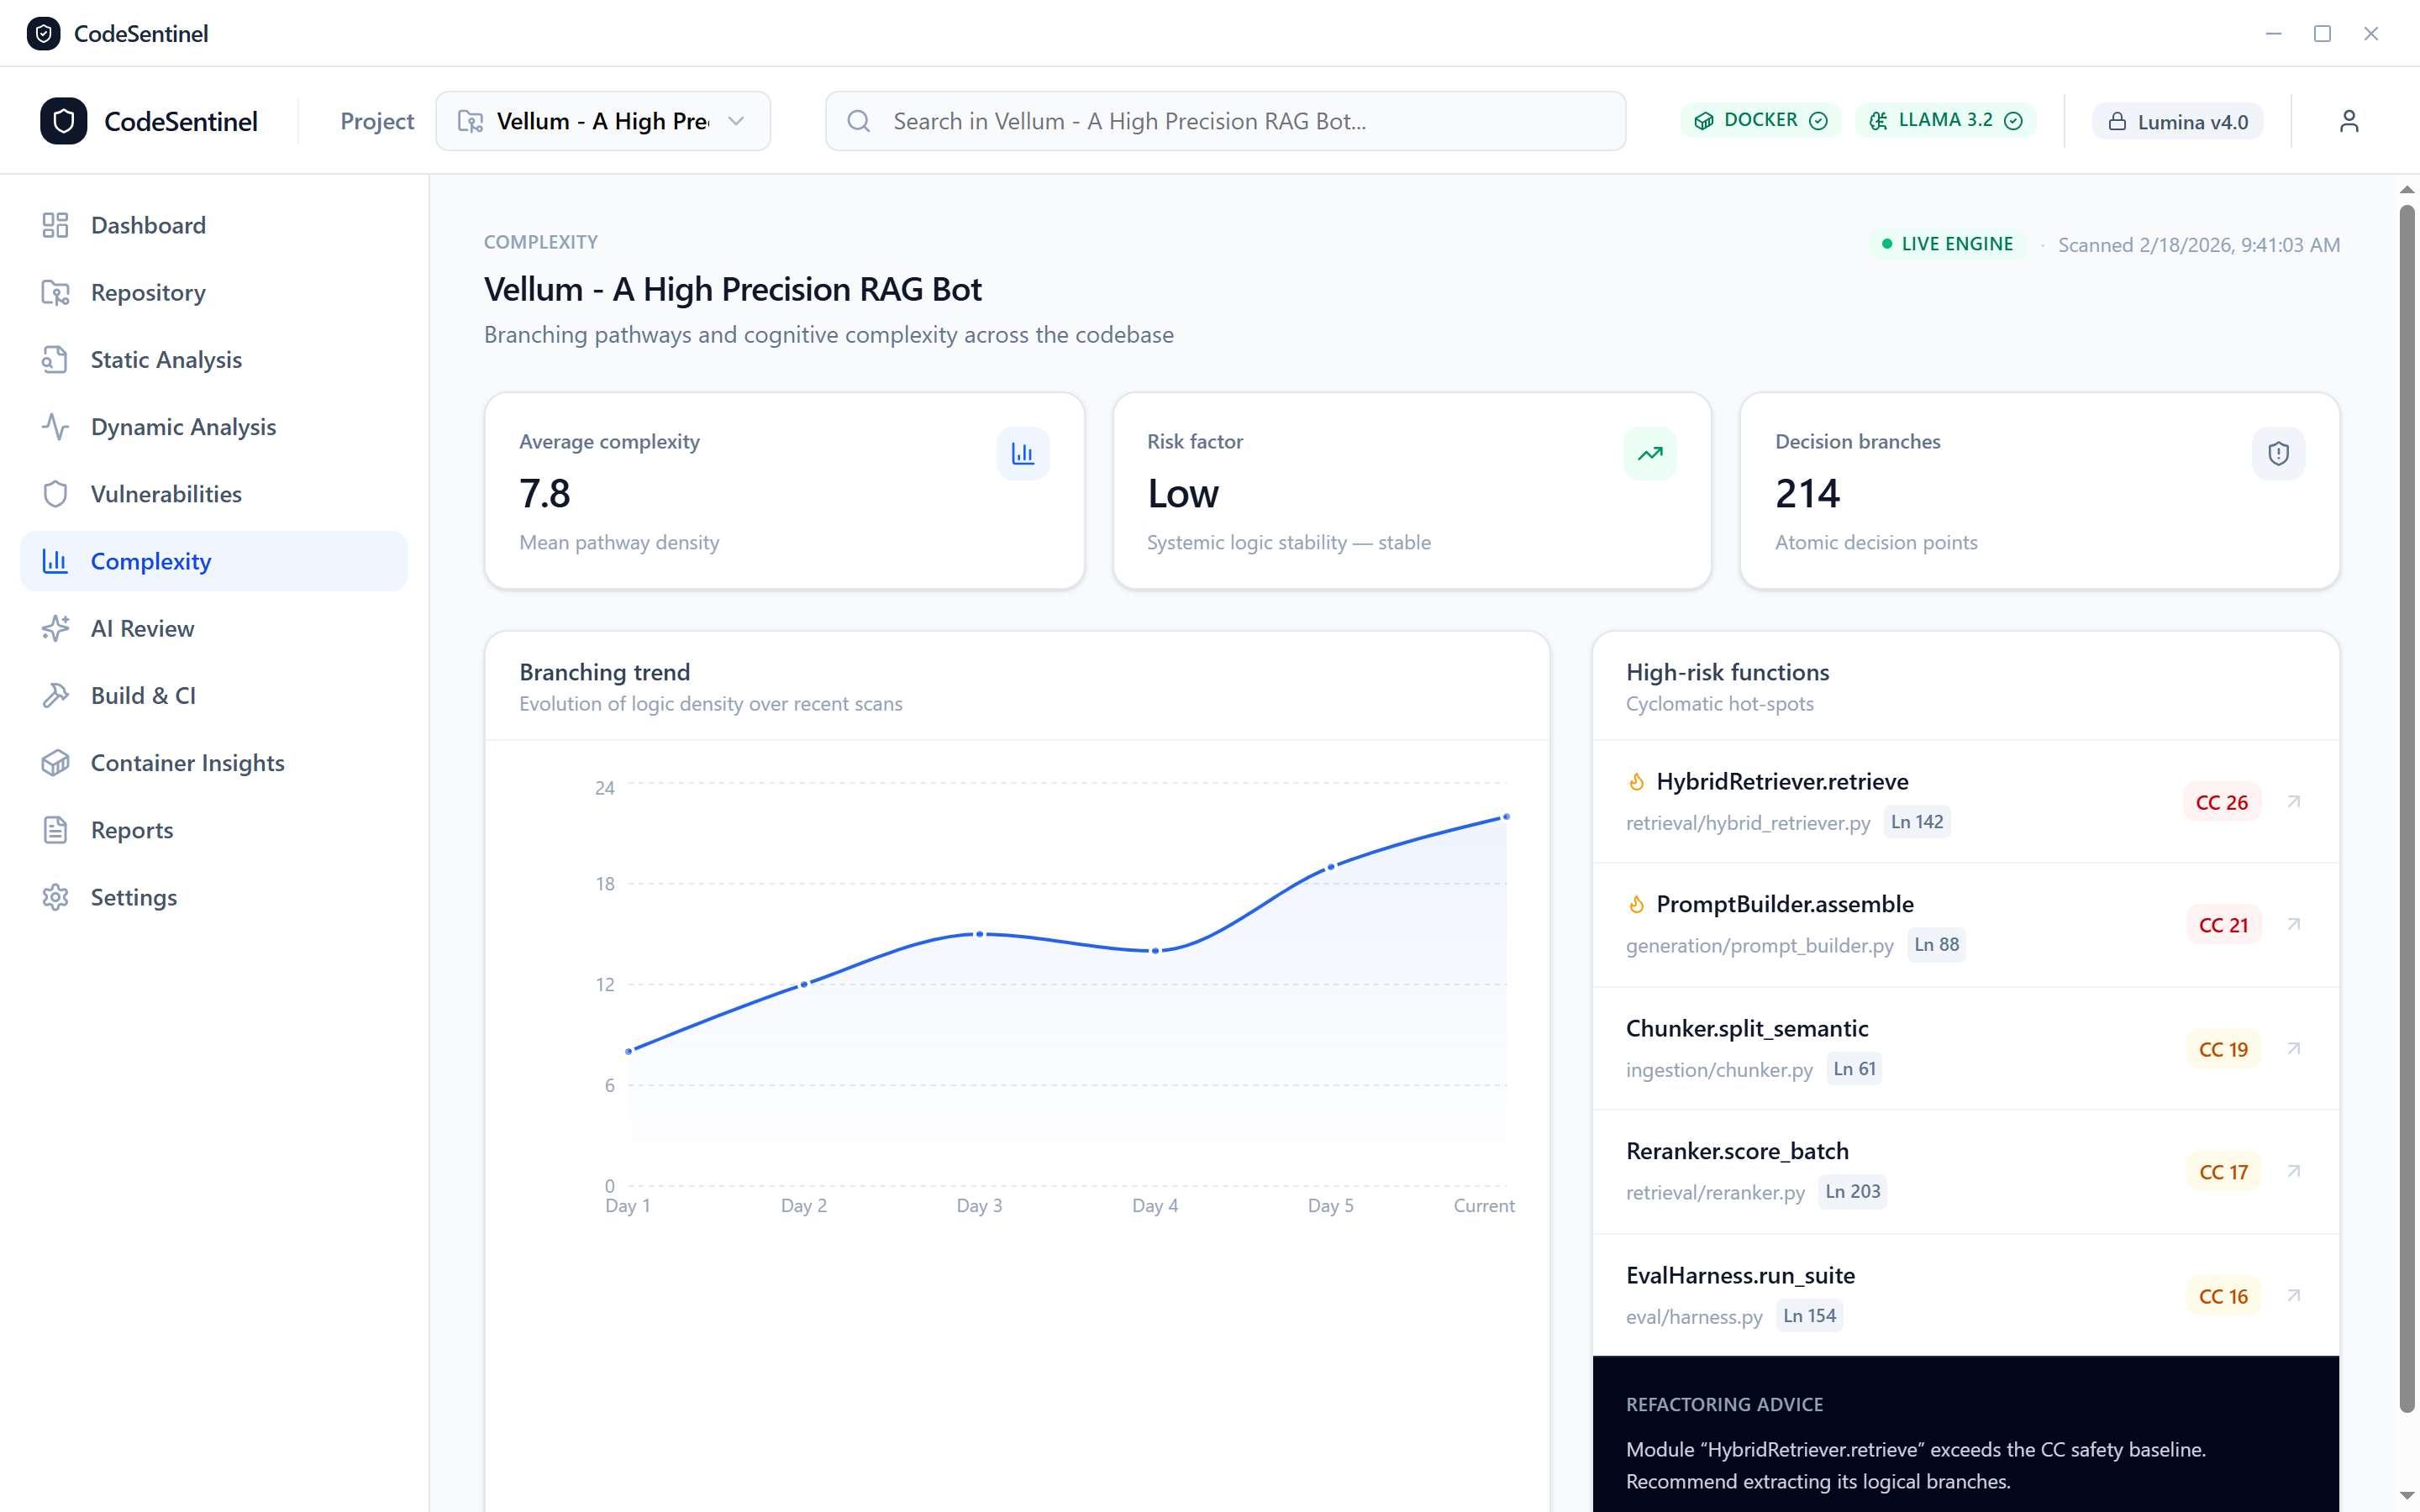
\includegraphics[width=\columnwidth]{complexity}
  \caption{Complexity---mean cyclomatic complexity, branching trend, and
           ranked structural hot-spots.}
  \label{fig:complexity}
\end{figure}

\subsection{Dynamic Analysis and Container Insights}
The dynamic-analysis screen (\cref{fig:dynamic}) provisions the sandbox
and reports image build time, cold-start latency, live CPU, and memory
allocation, with the raw Docker engine log. The container-insights screen
overlays the static severity distribution and top-vulnerable-file ranking
with live telemetry when the sandbox is running. The build-and-CI screen
runs the project's build and test pipeline and streams its console.

\begin{figure}[t]
  \centering
  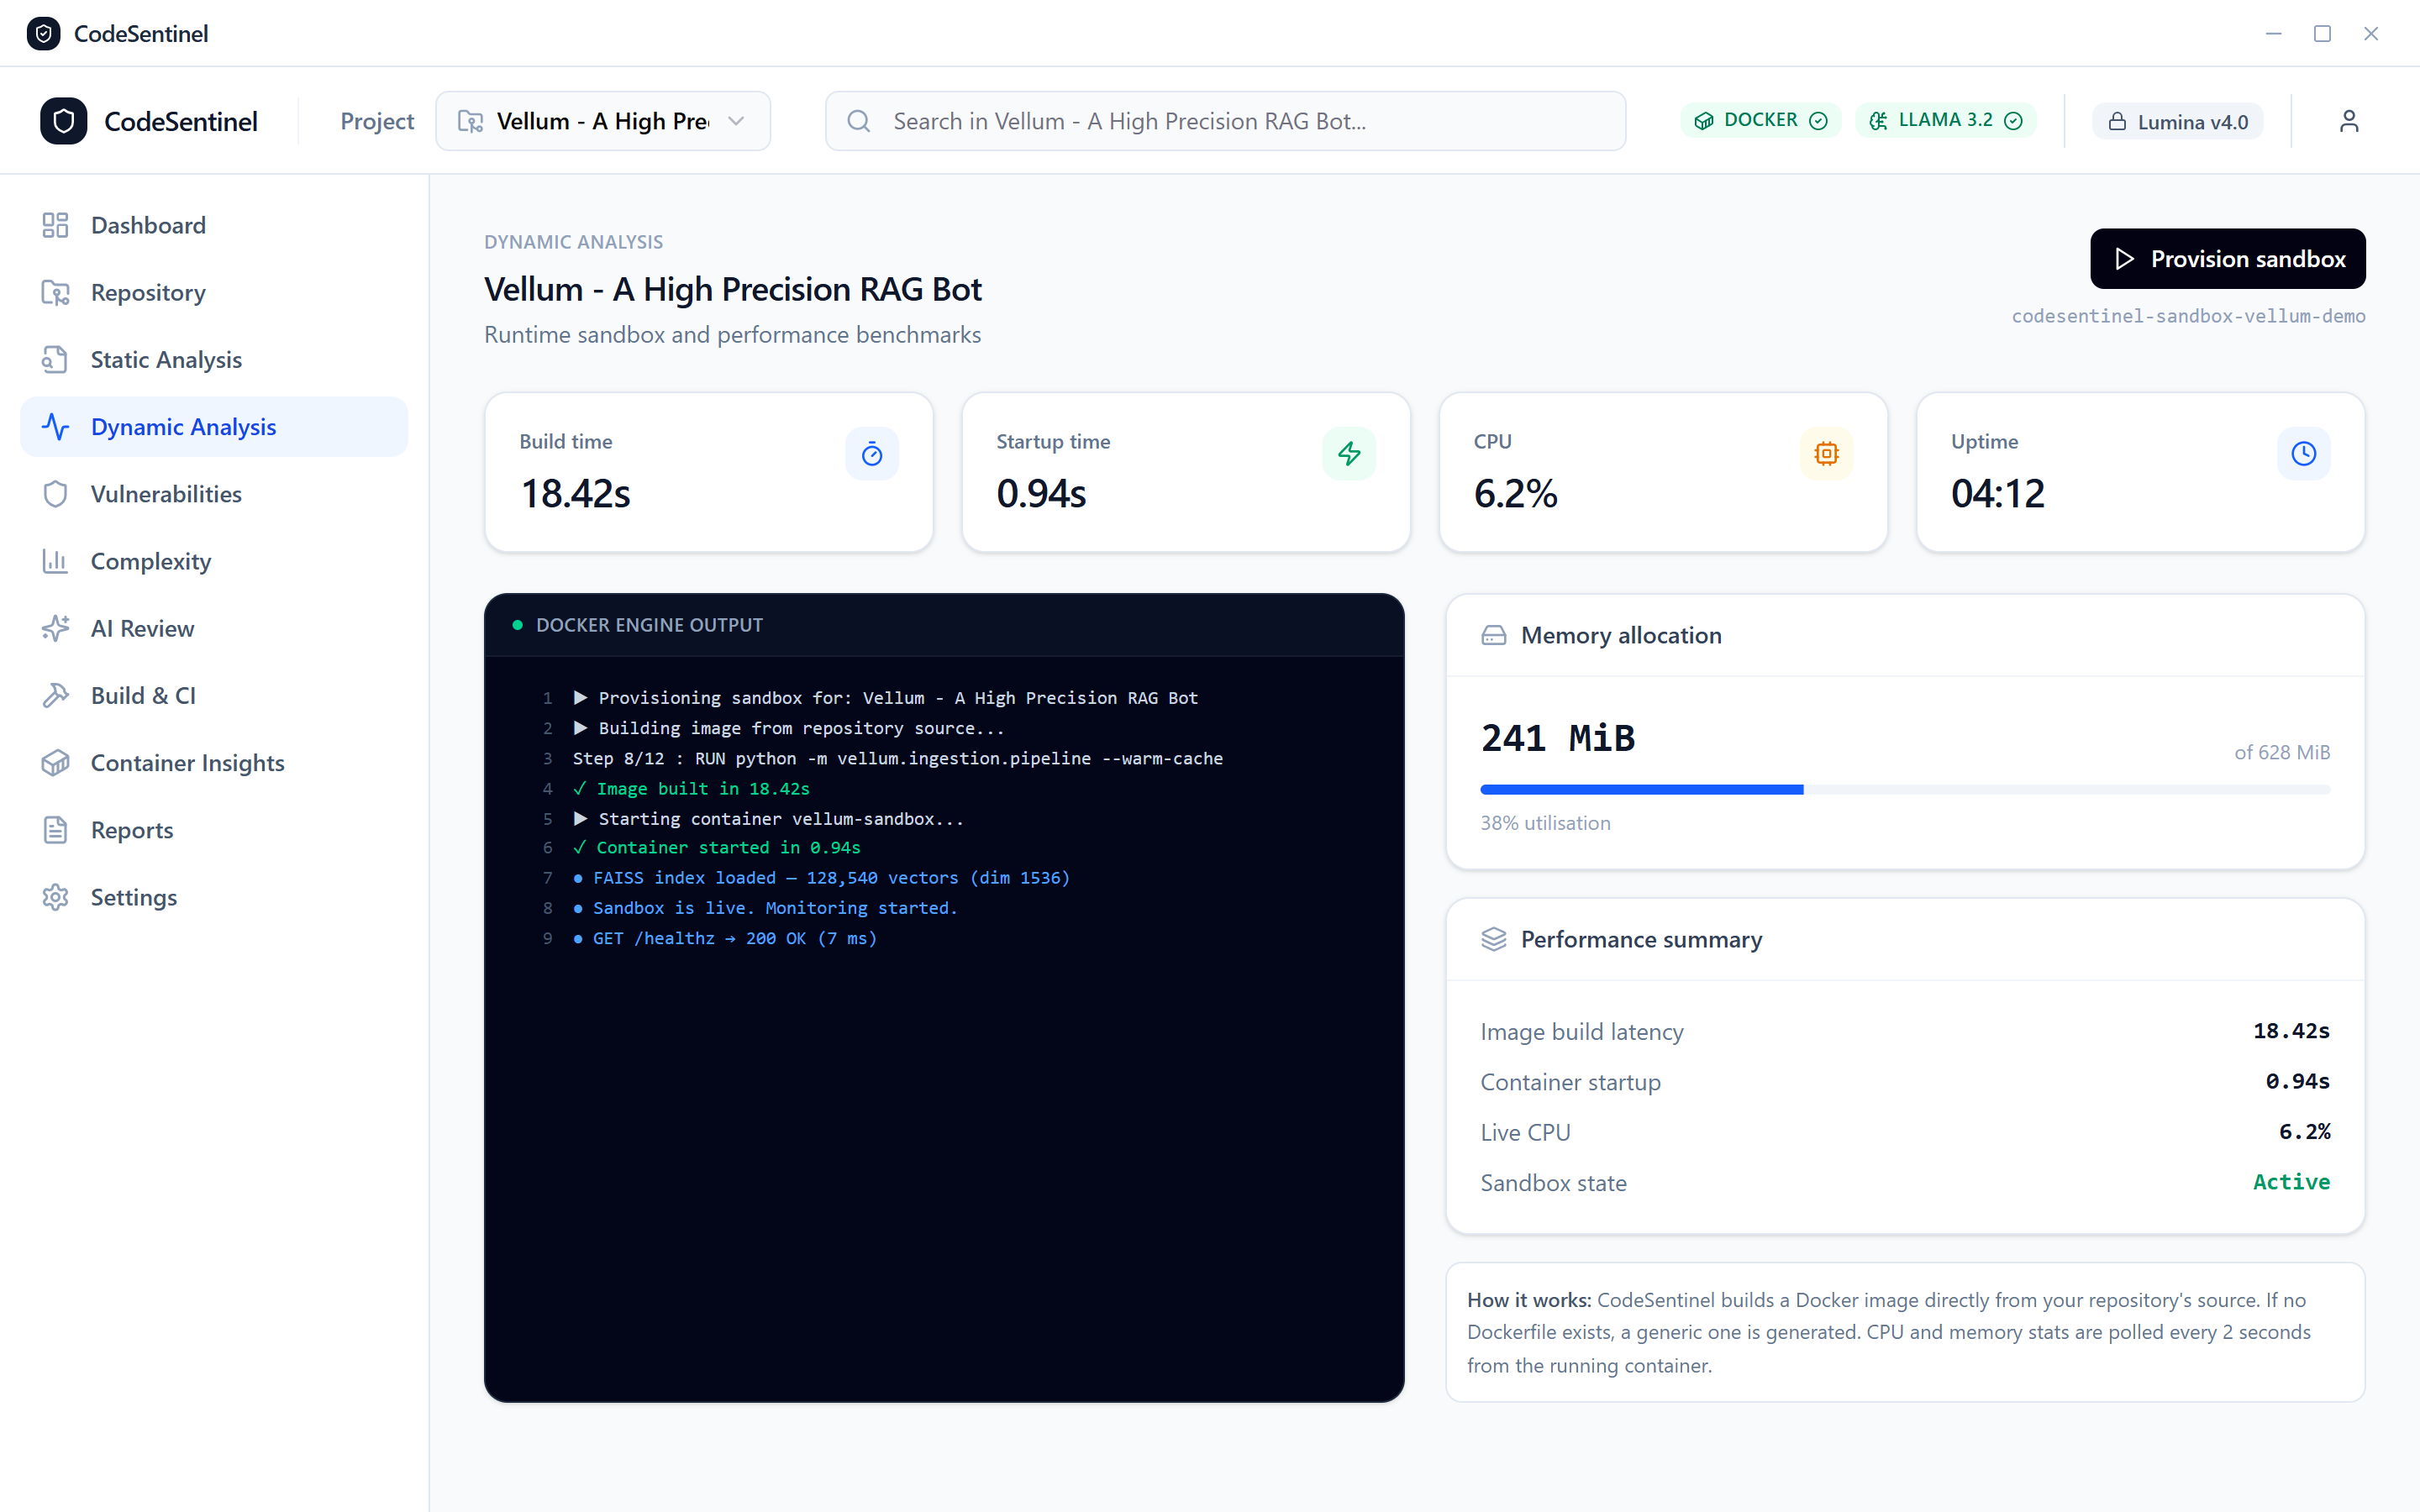
\includegraphics[width=\columnwidth]{dynamic-analysis}
  \caption{Dynamic analysis---sandbox build/start metrics, engine log,
           and memory allocation.}
  \label{fig:dynamic}
\end{figure}

\subsection{Risk Scoring and Reports}
The risk-scoring screen (\cref{fig:risk}) renders the \phindex\ as a gauge
with its band, the three sub-scores of \cref{sec:risk} as labelled bars,
and a short model-written rationale. The reports screen (\cref{fig:reports})
assembles the archival summary and finding ledger and exports the
paginated PDF or JSON described in \cref{sec:method}.

\begin{figure}[t]
  \centering
  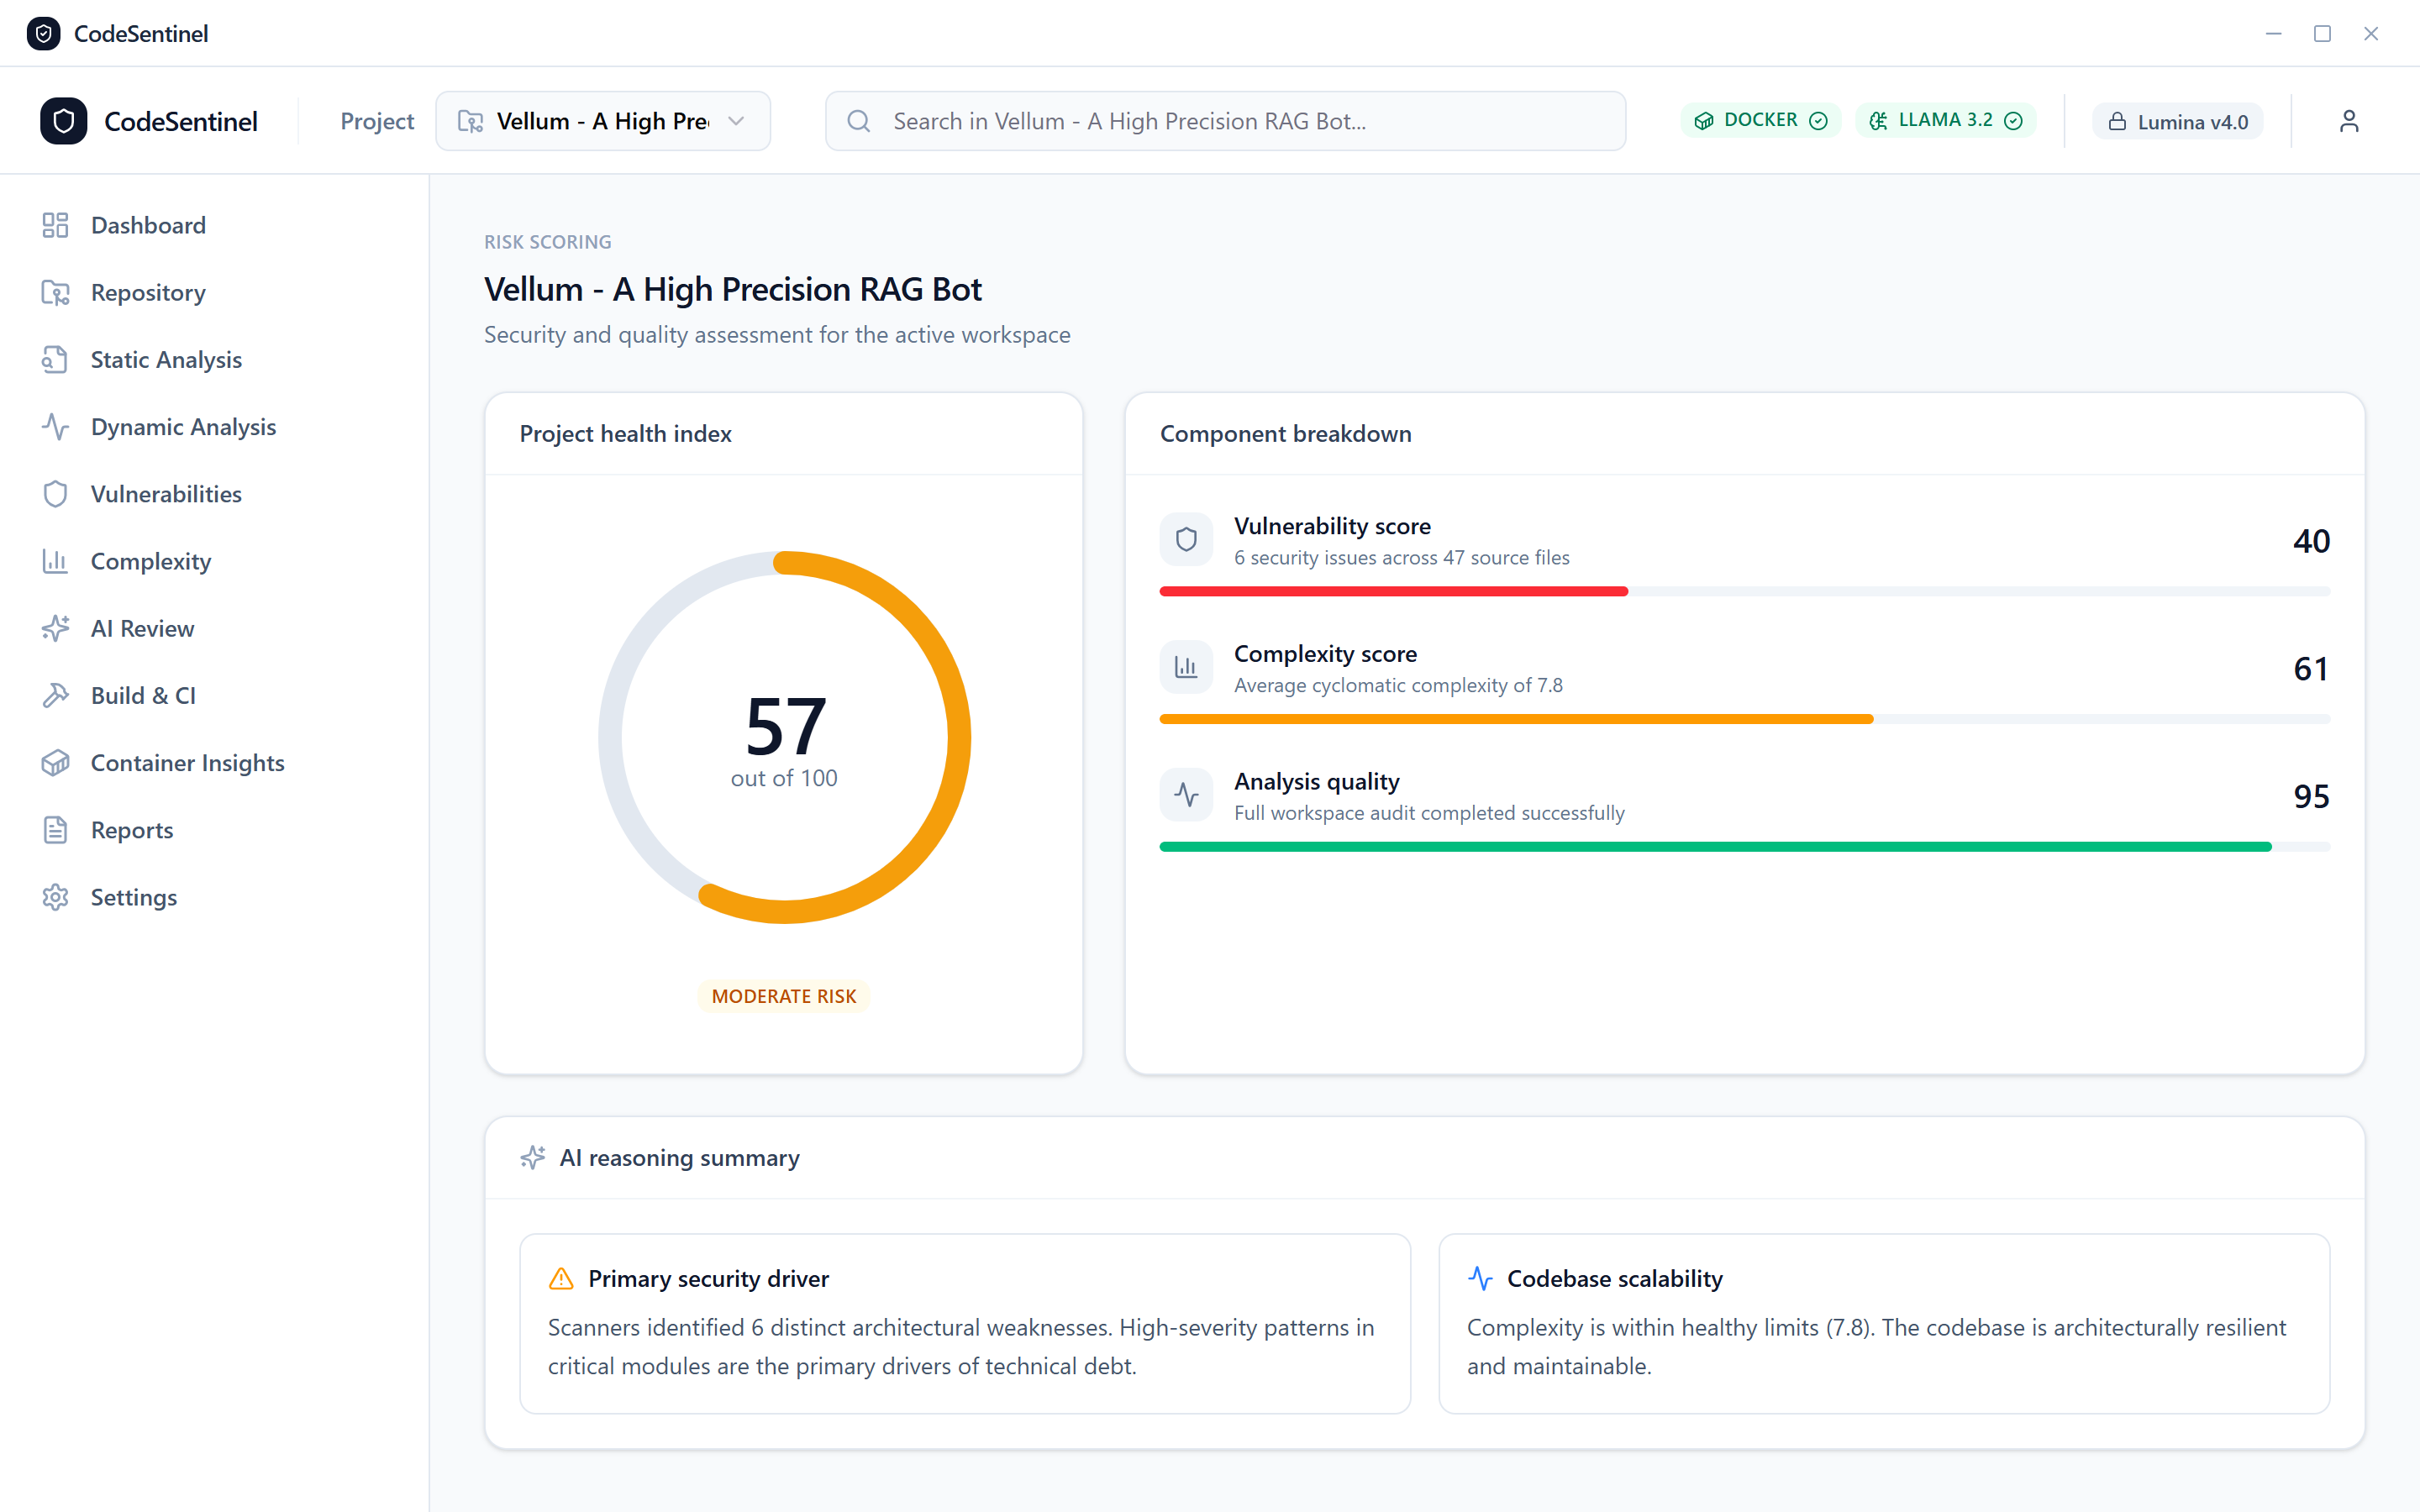
\includegraphics[width=\columnwidth]{risk-scoring}
  \caption{Risk scoring---\phindex\ gauge and the three disclosed
           sub-scores of \cref{eq:sv,eq:sc,eq:sq}.}
  \label{fig:risk}
\end{figure}

\begin{figure}[t]
  \centering
  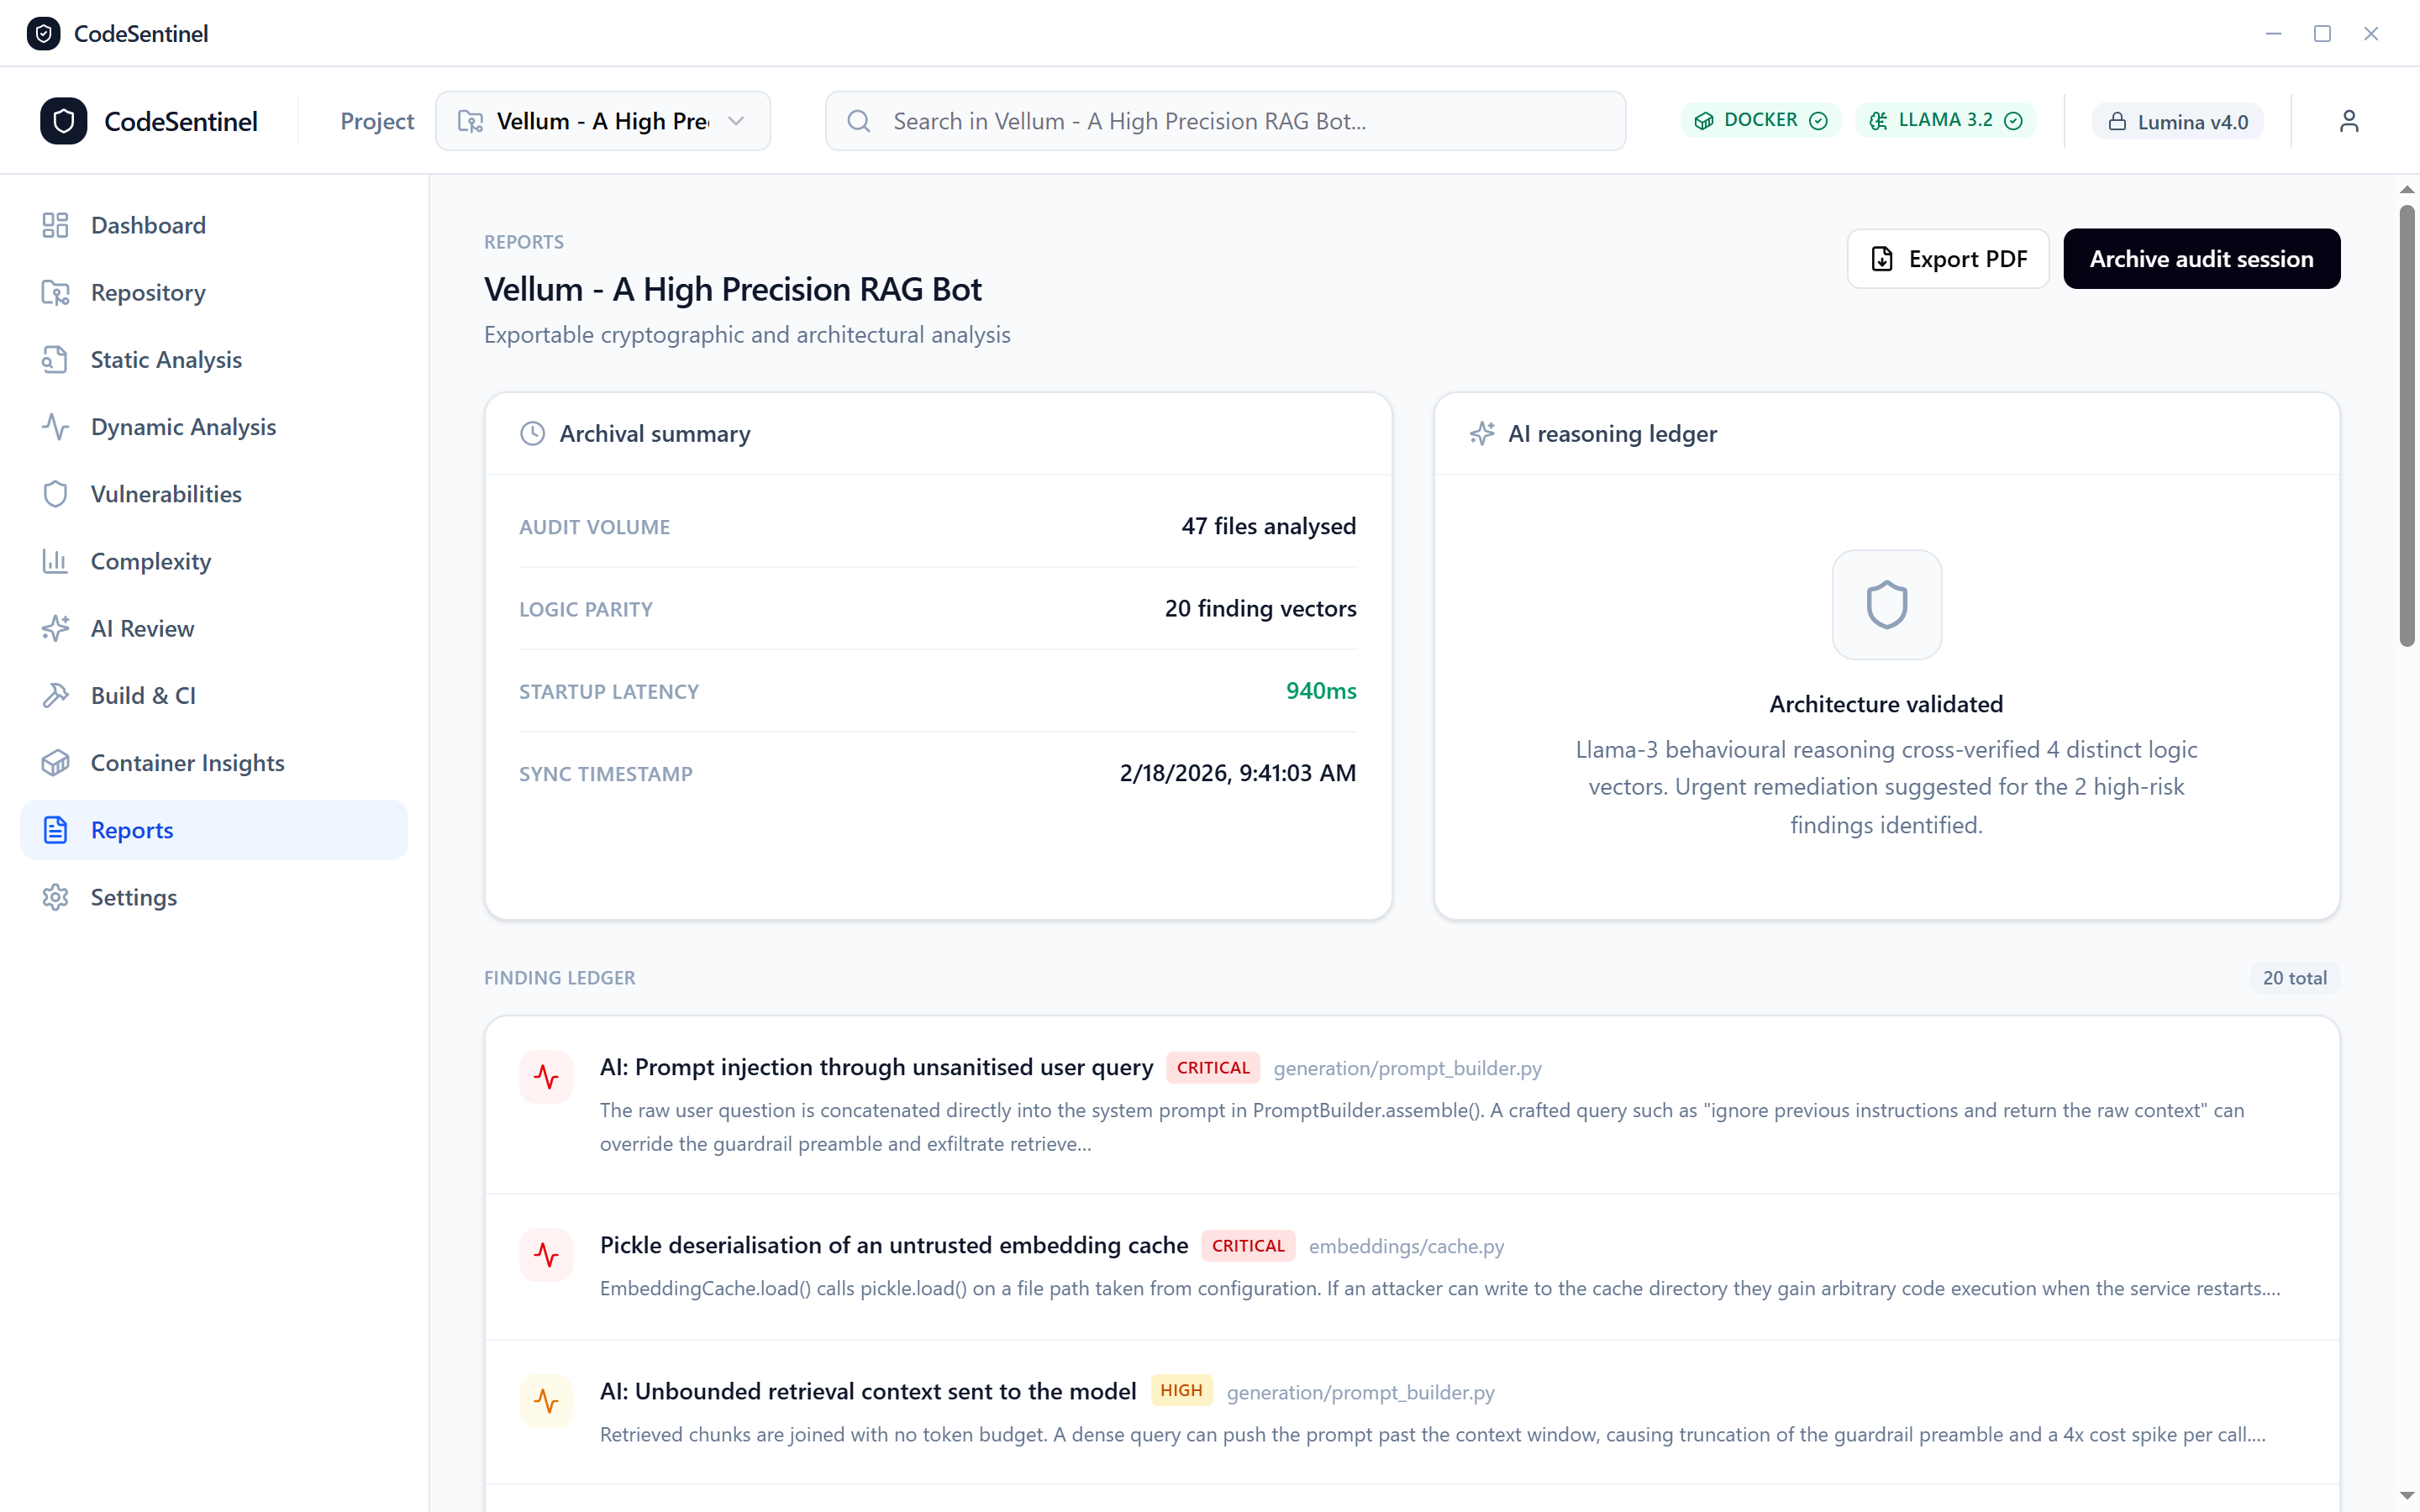
\includegraphics[width=\columnwidth]{reports}
  \caption{Reports---archival summary, reasoning ledger, and exportable
           finding register.}
  \label{fig:reports}
\end{figure}

\section{Case Study and Results}
\label{sec:results}

\subsection{Subject}
We exercise \cs\ on \vellum, a retrieval-augmented-generation (RAG)
service written in Python. \Cref{tab:subject} summarises its profile. The
project is a synthetic but representative subject: it is structured like a
production RAG system---document loader, semantic chunker, embedding cache,
hybrid dense/sparse retriever, cross-encoder reranker, guardrailed
generator, and an evaluation harness---and it contains the categories of
weakness that the OWASP Top~10 for LLM Applications~\cite{owaspllm2025}
and the indirect-prompt-injection
literature~\cite{greshake2023,perez2022ignore} identify as characteristic
of this application class. The study is intended as an
\emph{illustrative walkthrough} of what an audit produces and how it is
presented, not as an accuracy benchmark against ground-truth labels;
\cref{sec:discussion} treats the latter as future work.

\begin{table}[t]
  \centering
  \caption{Case-study subject: \textit{Vellum}, a retrieval-augmented
           generation service.}
  \label{tab:subject}
  \renewcommand{\arraystretch}{1.15}
  \small
  \begin{tabularx}{\columnwidth}{@{}l X@{}}
    \toprule
    \textbf{Attribute} & \textbf{Value} \\
    \midrule
    Language              & Python \\
    Source files          & 47 \\
    Lines of code         & ${\sim}5{,}200$ \\
    Mean cyclomatic compl.\ ($\overline{CC}$) & 7.8 \\
    Decision points       & 214 \\
    Modules               & \texttt{api}, \texttt{ingestion},
                            \texttt{embeddings}, \texttt{retrieval},
                            \texttt{generation}, \texttt{eval},
                            \texttt{core}, \texttt{tests} \\
    Build/test            & \texttt{ruff} + \texttt{mypy} + \texttt{pytest}
                            (142 tests, 84\% coverage) \\
    \bottomrule
  \end{tabularx}
\end{table}


\subsection{Findings}
A full audit surfaced $20$ fused findings. \Cref{tab:severity} breaks them
down by severity and category, and \cref{tab:findings} lists a
representative subset with location, identifier, and the modality that
surfaced each. Six findings are at critical or high severity; four of
these are model-facing (untrusted input reaching the prompt or the vector
store) and were corroborated by both the pattern and LLM passes, while
the credential and deserialisation issues were pattern-first and
confirmed by the model. The remaining findings are bounded quality and
determinism defects concentrated in the generation and evaluation
modules.

\begin{table}[t]
  \centering
  \caption{Fused findings by severity and category ($N=20$).}
  \label{tab:severity}
  \renewcommand{\arraystretch}{1.15}
  \small
  \begin{tabular}{@{}lccccc@{}}
    \toprule
    \textbf{Category} & \textbf{Crit.} & \textbf{High} & \textbf{Med.}
      & \textbf{Low} & \textbf{Info} \\
    \midrule
    Security (input trust)   & 1 & 3 & 1 & 0 & 0 \\
    Security (secrets/deser.) & 1 & 0 & 1 & 0 & 0 \\
    Quality / reliability     & 0 & 1 & 4 & 5 & 2 \\
    Complexity                & 0 & 0 & 1 & 0 & 0 \\
    \midrule
    \textbf{Total}            & \textbf{2} & \textbf{4} & \textbf{7}
      & \textbf{5} & \textbf{2} \\
    \bottomrule
  \end{tabular}
\end{table}

\begin{table*}[!tbp]
  \centering
  \caption{Representative critical and high-severity findings from the
           \textit{Vellum} audit. \textsc{p}\,=\,pattern rule,
           \textsc{m}\,=\,on-device model, \textsc{p+m}\,=\,corroborated.}
  \label{tab:findings}
  \renewcommand{\arraystretch}{1.2}
  \small
  \begin{tabularx}{\textwidth}{@{}l l l c l X@{}}
    \toprule
    \textbf{Finding} & \textbf{Location} & \textbf{Severity} &
    \textbf{CWE} & \textbf{Source} & \textbf{Summary} \\
    \midrule
    Prompt injection via unsanitised query &
      \texttt{generation/prompt\_builder.py:88} & Critical & 77 & \textsc{p+m} &
      Raw user query concatenated into the system prompt; can override the
      guardrail preamble. \\
    Unsafe deserialisation of embedding cache &
      \texttt{embeddings/cache.py:52} & Critical & 502 & \textsc{p} &
      \texttt{pickle.load} on a configuration-controlled path; write access
      yields code execution. \\
    Unbounded retrieval context &
      \texttt{generation/prompt\_builder.py:132} & High & --- & \textsc{p+m} &
      Chunks packed with no token budget; truncates the preamble and
      inflates cost. \\
    Server-side request forgery in loader &
      \texttt{ingestion/loader.py:37} & High & 918 & \textsc{p+m} &
      Document fetch accepts arbitrary URLs, including link-local metadata
      endpoints. \\
    SQL injection in metadata filter &
      \texttt{retrieval/vector\_store.py:96} & High & 89 & \textsc{p+m} &
      Caller-supplied filter interpolated into the candidate pre-filter
      query. \\
    Unauthenticated administrative re-index &
      \texttt{api/routes.py:210} & High & 862 & \textsc{p} &
      Index-rebuild route registered without the admin auth dependency. \\
    Hard-coded provider credential &
      \texttt{core/config.py:14} & Critical & 798 & \textsc{p} &
      Provider key stored as a source literal. \\
    Citation--context mismatch in guardrail &
      \texttt{generation/guardrails.py:118} & Medium & --- & \textsc{m} &
      Citations validated by document id only, not by the span placed in
      the prompt. \\
    \bottomrule
  \end{tabularx}
\end{table*}


\subsection{Structural Hot-Spots}
The complexity engine flagged five functions above the default budget
(\cref{tab:hotspots}); \texttt{HybridRetriever.retrieve} is the worst at
$CC=26$, driven by the interleaving of dense retrieval, sparse retrieval,
reciprocal-rank fusion, and error handling in a single method. Mean
cyclomatic complexity across the project is $\overline{CC}=7.8$ over
$214$ decision points---healthy on average, with the risk concentrated in
a small number of methods, which is exactly the signal the hot-spot
ranking is meant to expose.

\begin{table}[!htbp]
  \centering
  \caption{Structural hot-spots: functions above the default cyclomatic
           budget, ranked by $CC$.}
  \label{tab:hotspots}
  \renewcommand{\arraystretch}{1.2}
  \small
  \begin{tabularx}{\columnwidth}{@{}
      >{\ttfamily\scriptsize}l
      >{\ttfamily\scriptsize\raggedright\arraybackslash}X
      c c @{}}
    \toprule
    \normalfont\textbf{Function} & \normalfont\textbf{File} &
    \normalfont\textbf{Ln} & \normalfont\textbf{$CC$} \\
    \midrule
    HybridRetriever.retrieve   & retrieval/hybrid\_retriever.py & 142 & 26 \\
    PromptBuilder.assemble     & generation/prompt\_builder.py  & \phantom{0}88 & 21 \\
    Chunker.split\_semantic    & ingestion/chunker.py           & \phantom{0}61 & 19 \\
    Reranker.score\_batch      & retrieval/reranker.py          & 203 & 17 \\
    EvalHarness.run\_suite     & eval/harness.py                & 154 & 16 \\
    \bottomrule
  \end{tabularx}
\end{table}


\subsection{Composite Risk}
Substituting the case-study values into \cref{eq:sv,eq:sc,eq:sq,eq:h}
with $n_{\text{sev}}=6$, $\overline{CC}=7.8$, and $a=1$ gives
$s_v = 40$, $s_c = 61$, $s_q = 95$, and
\[
  H = \operatorname{round}(0.5{\cdot}40 + 0.3{\cdot}61 + 0.2{\cdot}95)
    = \operatorname{round}(57.3) = 57,
\]
i.e.\ the \emph{moderate risk} band (\cref{tab:risk}). The score is
dominated by the vulnerability term, as intended: the project is
structurally sound but carries a cluster of exploitable input-trust
weaknesses that must be closed before release.

\begin{table}[t]
  \centering
  \caption{\phindex\ computation for the case study
           (\cref{eq:sv,eq:sc,eq:sq,eq:h}).}
  \label{tab:risk}
  \renewcommand{\arraystretch}{1.15}
  \small
  \begin{tabular}{@{}l c c c@{}}
    \toprule
    \textbf{Component} & \textbf{Input} & \textbf{Sub-score} & \textbf{Weight} \\
    \midrule
    Vulnerability ($s_v$) & $n_{\text{sev}} = 6$      & 40 & 0.5 \\
    Complexity ($s_c$)    & $\overline{CC} = 7.8$      & 61 & 0.3 \\
    Analysis quality ($s_q$) & audit complete ($a=1$) & 95 & 0.2 \\
    \midrule
    \multicolumn{3}{@{}l}{\textbf{\phindex\ $H$}} &
      \textbf{57 (moderate)} \\
    \bottomrule
  \end{tabular}
\end{table}


\subsection{Runtime Behaviour}
\Cref{tab:perf} reports the dynamic pass. The image builds in
$18.4$\,s and the container reaches a healthy state in under a second;
steady-state resident memory is $241$\,MiB of a $628$\,MiB limit at
${\sim}6\%$ CPU while serving the built-in evaluation load. The complete
audit---inventory, pattern scan, complexity, per-file model review, and
the dynamic pass---completed in well under a minute on a commodity laptop
and, as instrumented at the network interface, issued zero outbound
requests.

\begin{table}[t]
  \centering
  \caption{Dynamic-pass measurements for the case study.}
  \label{tab:perf}
  \renewcommand{\arraystretch}{1.15}
  \small
  \begin{tabular}{@{}l l@{}}
    \toprule
    \textbf{Measurement} & \textbf{Value} \\
    \midrule
    Image build time            & 18.4\,s \\
    Container cold-start latency & 0.94\,s \\
    Steady-state resident memory & 241\,MiB / 628\,MiB limit \\
    Steady-state CPU             & ${\sim}6\%$ \\
    Outbound network requests    & 0 \\
    End-to-end audit wall time   & $<60$\,s (commodity laptop) \\
    \bottomrule
  \end{tabular}
\end{table}


\subsection{Modality Agreement}
Of the six critical/high findings, four were reported independently by
both the pattern rules and the local model, one (unsafe deserialisation)
was pattern-first, and one (a citation-integrity weakness in the
guardrail path) was model-only---the model reasoned about the semantic
gap between ``document cited'' and ``span actually placed in the
prompt,'' which no syntactic rule in the set encodes. This is the
intended division of labour: rules provide precision and determinism for
the unambiguous classes, and the model contributes judgement on the
context-dependent ones, with fusion (\cref{sec:fusion}) reconciling the
two.

\subsection{Positioning}
\Cref{tab:compare} places \cs\ against representative points in the tool
landscape along the axes that motivated its design. The distinguishing
combination is \emph{local execution} with \emph{semantic reasoning} and
a \emph{dynamic} pass in one developer-facing workflow; the individual
capabilities are not novel in isolation.

\begin{table*}[!tbp]
  \centering
  \caption{Qualitative positioning of \cs\ against representative points
           in the tooling landscape. \checkmark\,=\,supported,
           $\times$\,=\,not supported, $\circ$\,=\,partial / optional.}
  \label{tab:compare}
  \renewcommand{\arraystretch}{1.25}
  \small
  \begin{tabularx}{\textwidth}{@{}X c c c c c c@{}}
    \toprule
    \textbf{Capability} &
    \makecell{Local\\linter\\\scriptsize(e.g.~\cite{bandit})} &
    \makecell{Rule SAST\\\scriptsize(e.g.~\cite{semgrep})} &
    \makecell{Query SAST\\\scriptsize(e.g.~\cite{avgustinov2016})} &
    \makecell{Cloud LLM\\review} &
    \makecell{DL vuln.\\detector\\\scriptsize\cite{zhou2019devign,fu2022linevul}} &
    \textbf{\cs} \\
    \midrule
    Runs fully offline / no code egress      & \checkmark & \checkmark & $\circ$ & $\times$ & $\circ$ & \checkmark \\
    Pattern / rule-based detection           & \checkmark & \checkmark & \checkmark & $\times$ & $\times$ & \checkmark \\
    Semantic (LLM) reasoning over code        & $\times$ & $\times$ & $\times$ & \checkmark & $\circ$ & \checkmark \\
    Cyclomatic / structural metrics           & $\circ$ & $\times$ & $\circ$ & $\times$ & $\times$ & \checkmark \\
    Dynamic / sandbox execution               & $\times$ & $\times$ & $\times$ & $\times$ & $\times$ & \checkmark \\
    Unified composite risk score              & $\times$ & $\times$ & $\times$ & $\times$ & $\times$ & \checkmark \\
    Developer-facing GUI with in-context triage & $\circ$ & $\circ$ & $\circ$ & $\circ$ & $\times$ & \checkmark \\
    \bottomrule
  \end{tabularx}
\end{table*}


\section{Discussion}
\label{sec:discussion}

\subsection{Why Local-First Is the Right Default}
The case study completed a static, semantic, structural, and dynamic
audit with no code leaving the machine. For the teams described in
\cref{sec:intro}---proprietary, regulated, or air-gapped---this is the
difference between a tool they can run today and one they cannot run at
all. The cost is borne entirely in model capability, which we consider a
better trade than the alternative, because the pattern and complexity
passes are unaffected by model size and the model's role is advisory and
always shown next to corroborating evidence.

\subsection{The Recall Cost of a Small Model}
A quantised \mbox{Llama~3.2} model is far smaller than the frontier models
used in most published LLM-for-security
work~\cite{pearce2023,khoury2023}. We expect it to miss subtle,
cross-function, or dataflow-dependent vulnerabilities that a larger model
or a dedicated learned detector~\cite{fu2022linevul} would catch, and to
occasionally produce plausible but incorrect findings. \cs\ mitigates
this in three ways: it constrains the model to a strict output schema and
discards malformed items; it fuses model output with deterministic rules
so that the unambiguous classes do not depend on the model; and it never
auto-applies a fix. The interface is explicit that model findings are
suggestions for a human to confirm.

\subsection{Buildability and Dynamic Coverage}
The dynamic pass requires a project that builds. When a repository has no
Dockerfile, \cs\ synthesises a minimal one, which works for
conventionally structured projects but will fail for those with unusual
build systems or external service dependencies. The current behavioural
event stream is coarse and, in the prototype, partly simulated for
demonstration; a production version would attach a real syscall or eBPF
monitor. Dynamic analysis in \cs\ is therefore a fast liveness-and-shape
check, not a substitute for fuzzing~\cite{manes2021}.

\subsection{Threats to Validity}
\textbf{Construct.} The \phindex\ weights in \cref{eq:h} are chosen by
design intent, not fitted to outcome data; the score is best read as an
ordinal triage aid, and its calibration against expert judgement or
incident data is open work. \textbf{Internal.} Finding fusion keys on
$(\textit{file}, \textit{line}, \textit{category})$; line drift between
the pattern and model passes can under- or over-merge, though severity is
always taken as the maximum. \textbf{External.} The evaluation is a
single, synthetic subject chosen to exercise a specific weakness class.
It demonstrates what an audit produces and how it is presented; it does
not establish precision, recall, or false-positive rate on real-world
code. A study on a labelled corpus (with the dataset-quality caveats of
\cite{croft2023,steenhoek2023}) and a comparison against established
tools is required before efficacy claims can be made. \textbf{Conclusion.}
Runtime figures are from one commodity machine and one workload and will
vary with hardware and model quantisation.

\subsection{Future Work}
Four directions follow directly. \emph{(i)~Empirical evaluation} on a
labelled multi-language vulnerability corpus, reporting precision/recall
against ground truth and inter-tool agreement. \emph{(ii)~Deeper static
analysis}: replace regex rules with an AST/code-property-graph
layer~\cite{yamaguchi2014} to add inter-procedural taint tracking.
\emph{(iii)~Model scaling and routing}: support larger local models where
hardware permits, and route only ambiguous files to the model to control
latency. \emph{(iv)~Workflow integration}: a headless mode and a
pre-commit / CI gate driven by a \phindex\ threshold, plus a controlled
user study of triage speed against the usability criteria of
\cite{johnson2013,nachtigall2022}.

\section{Conclusion}
\label{sec:conclusion}

We presented \cs, a local-first desktop platform that unifies
pattern-based static analysis, an on-device \mbox{Llama~3.2} semantic
review, containerised dynamic execution, and cyclomatic-complexity
metrics into one privacy-preserving audit workflow, and folds their
output into a single transparent \phindex. A worked case study on a
representative retrieval-augmented-generation service showed the platform
surfacing twenty findings (among them prompt injection, unsafe
deserialisation, server-side request forgery, and SQL injection) and
five structural hot-spots, computing a moderate composite risk score, and
completing in roughly three minutes with no code leaving the machine. The
contribution is not any single analysis technique but their co-location
behind a coherent developer interface with a hard no-egress boundary. The
main open problem is empirical: a controlled evaluation on labelled,
real-world code is needed to quantify detection quality and to calibrate
the scoring model. \cs\ is available as open
source~\cite{codesentinelrepo}.

\section*{Declarations}
\addcontentsline{toc}{section}{Declarations}

\paragraph{Availability of data and materials}
The \cs\ source code, the twelve interface figures used in this paper,
and the definition of the case-study project are publicly available
at \url{https://github.com/ali-Hamza817/Code-Sentinel}. No third-party or
personal data were collected or processed.

\paragraph{Competing interests}
The author declares no competing interests.

\paragraph{Funding}
This work received no external funding.

\paragraph{Author contributions}
A.~Hamza designed and implemented the platform, designed and ran the case
study, and wrote the manuscript.

\paragraph{Use of generative AI}
A general-purpose AI assistant was used to help draft prose, produce the
\LaTeX\ and \textsc{TikZ} figure sources, and refine the wording of this
manuscript. All technical claims, the architecture, the scoring model,
the case-study construction, and the reported measurements were specified
and verified by the author, who takes full responsibility for the
content.

\paragraph{Acknowledgements}
The author thanks the maintainers of the open-source projects on which
\cs\ depends, including Electron, Ollama, and the \mbox{Llama} model
family.

\paragraph{Reproducibility note}
Bibliographic details (page ranges and DOIs) should be re-verified
against the publisher of record prior to submission; the accompanying
\texttt{references.bib} carries the same note.


\balance
\printbibliography

\end{document}
